%\documentclass[a4paper]{article}
% #### CONFIGURACIONES ####
\documentclass[12pt,a4paper,oneside]{book} % tamaño 12
%\usepackage[spanish]{babel}
\usepackage[spanish, es-tabla]{babel}
\usepackage[utf8x]{inputenc}
\usepackage[pass]{geometry}
\usepackage[usenames]{color}
\usepackage[table,xcdraw]{xcolor}
\usepackage{tikz} % grafos
\usetikzlibrary{arrows,shapes,positioning,shadows,trees}
\usepackage{amsmath} % códigos
\usepackage{setspace} %interlineado algoritmo
\usepackage{algorithm}
%\usepackage{algorithmicx}
\usepackage{algpseudocode}
\usepackage{rotating} % rotate graphics
\usepackage{pdflscape} % automatic rotation of the page 
\usepackage{longtable}
\algdef{SE}[DOWHILE]{Do}{doWhile}{\algorithmicdo}[1]{\algorithmicwhile\ #1}%
\usepackage[hidelinks]{hyperref}
\usepackage{subfig} % Para poner imágenes
\usepackage{graphicx} % para poner dos imágenes juntas
\usepackage[colorinlistoftodos]{todonotes}
\usepackage{anysize}
\marginsize{4cm}{2.5cm}{2.5cm}{2.5cm}
% Márgenes {izquierda}{derecha}{arriba}{abajo}.
\usepackage{mathptmx}% http://ctan.org/pkg/mathptmx Times new roman
\usepackage{amsfonts}% Para expresiones matemáticas
%\usepackage{setspace} % interlineado
\renewcommand{\baselinestretch}{1.5} % Interlineado
\usepackage{enumerate}% para los enumerate
\usepackage{fancyhdr}
\pagestyle{fancy}
\usepackage[none]{hyphenat} %saltos y justificación texto
\usepackage{float}
\usepackage{tikz}
\usetikzlibrary{calc}
\usepackage{changepage}
\usepackage{ragged2e}
\usepackage{tabularx} % Para meter tablas que no excedan los márgenes del papel
\usepackage{fancyhdr}
%%%%%%%%%%%%%%%%%%%%%%%
%%%%%%%% XML %%%%%%%%%%
\usepackage{listings}

\usepackage{appendix}
% cambiar apéndices por anexos
\renewcommand{\appendixname}{Anexos}
\renewcommand{\appendixtocname}{Anexos}
\renewcommand{\appendixpagename}{Anexos}
%\newcommand{\specialcell}[1]{\begin{tabular}{@{}c@{}}#1\end{tabular}}
 \everycr={\noalign{\global\advance\stepno by 1}}%
 
\usepackage{color}
\definecolor{gray}{rgb}{0.4,0.4,0.4}
\definecolor{darkblue}{rgb}{0.0,0.0,0.6}
\definecolor{cyan}{rgb}{0.0,0.6,0.6}

\usepackage[export]{adjustbox} % -- imagenes y cosas
\usepackage{enumitem}
\newlist{tabitemize}{itemize}{1}
\setlist[tabitemize]{label=\textbullet,nosep,after=\strut,align=parleft,leftmargin=*,}

\lstset{
  basicstyle=\ttfamily,
  columns=fullflexible,
  showstringspaces=false,
  commentstyle=\color{gray}\upshape
}

\lstdefinelanguage{XML}
{
  morestring=[b]",
  morestring=[s]{>}{<},
  morecomment=[s]{<?}{?>},
  stringstyle=\color{black},
  identifierstyle=\color{darkblue},
  keywordstyle=\color{cyan},
  morekeywords={id,tx,ty,tz,rx,ry,rz,scale,file,type}% list your attributes here
}
%%%%%%%%%%%%%%%%%%%%%%%%%%%%
%%%%%%%%%%%%% COLOR %%%%%%%%
\definecolor{palegreen}{rgb}{0.6, 0.98, 0.6}
\definecolor{palegoldenrod}{rgb}{0.93, 0.91, 0.67}

\makeatletter
\def\BState{\State\hskip-\ALG@thistlm}
\makeatother

%%%% Carpeta de las figuras

% Logo de la uex en el header de todas las páginas
%\rhead{\begin{picture}(0,0) \put(0,0){
\includegraphics[width=1cm,natwidth=124,natheight=163]{pictures/logouex_transp.png}}
%\end{picture}}
\fancypagestyle{plain}{
	\fancyhf{}
	\rhead{
\includegraphics[width=1cm,natwidth=124,natheight=163]{pictures/logouex_transp.png}}
	\fancyhead[L]{\leftmark}
	\headsep = -1cm
}
\pagestyle{fancy}
\fancyhf{}
\rhead{
\includegraphics[width=1cm,natwidth=124,natheight=163]{pictures/logouex_transp.png}}
\fancyhead[L]{\leftmark}
\headsep = 2cm
\begin{document}

\sloppy
\pagebreak
%http://tex.stackexchange.com/questions/129º088/create-a-frame-for-a-title-page
% ### DALE CAÑA PRIMO ###
\makeatletter
\begin{titlepage}
	\begin{adjustwidth}{-1.5cm}{0cm}
		\begin{tikzpicture}[remember picture, overlay]
		\usetikzlibrary{calc}
		\draw[line width = 1.5pt] ($(current page.north west) + (1in,-1in)$) rectangle ($(current page.south east) + (-1in,1in)$);
		\end{tikzpicture}

		\vspace{-3em}
		\hspace{-0.5em}
		\begin{minipage}{0.45\textwidth}
			\begin{flushleft}
				
\includegraphics[width=1.75cm,natwidth=124,natheight=163]{pictures/logouex_transp.png}
			\end{flushleft}
		\end{minipage}

		\vspace{-5.5em}
		\hspace{20em}
		\begin{minipage}{0.45\textwidth}
			\begin{flushright} % width=0.8\textwidth,height=0.8\textheight,keepaspectratio
				
\includegraphics[width=4cm, natwidth=233,natheight=135]{pictures/logoEpcc.png}
			\end{flushright}
		\end{minipage}\\[1.5cm]

		\begin{center}
			% Upper part of the page
			\textsc{\LARGE UNIVERSIDAD DE EXTREMADURA}\\[4cm]

			\textsc{\Large Escuela Politécnica}\\[0.5cm]
			\textsc{\Large Grado en Ingeniería Informática en Ingeniería de Software}\\[3cm]
			\textsc{\Large Trabajo Fin de Grado}\\[0.5cm]
%			{ \large \bfseries }\\[4.0cm]
			\vfill
			% Bottom of the page
			{\large}
		\end{center}
	\end{adjustwidth}
\end{titlepage}
\thispagestyle{empty}
\begin{titlepage}
	\begin{adjustwidth}{-1.5cm}{0cm}
		\begin{tikzpicture}[remember picture, overlay]
		\usetikzlibrary{calc}
		\draw[line width = 1.5pt] ($(current page.north west) + (1in,-1in)$) rectangle ($(current page.south east) + (-1in,1in)$);
		\end{tikzpicture}

		\vspace{-3em}
		\hspace{-0.5em}
		\begin{minipage}{0.55\textwidth}
			\begin{flushleft}
				
\includegraphics[width=1.75cm,natwidth=124,natheight=163]{pictures/logouex_transp.png}
			\end{flushleft}
		\end{minipage}

		\vspace{-5.5em}
		\hspace{20em}
		\begin{minipage}{0.45\textwidth}
			\begin{flushright}
				
\includegraphics[width=4cm,natwidth=233,natheight=135]{pictures/logoEpcc.png}
			\end{flushright}
		\end{minipage}\\[1.5cm]

		\begin{center}


			% Upper part of the page
			\textsc{\LARGE UNIVERSIDAD DE EXTREMADURA}\\[3cm]

			\textsc{\Large Escuela Politécnica}\\[0.5cm]
			\textsc{\Large Grado en Ingeniería Informática en Ingeniería de Software}\\[2.5cm]
			\textsc{\Large Trabajo Fin de Grado}\\[0.5cm]
			{ \large \bfseries Extracción del contexto de ejecución del usuario}\\[4.0cm]
			{ \large \bfseries Autor: Alberto de la Fuente Cruz}\\[0.5cm]
			{ \large \bfseries Tutor: Juan Manuel Murillo}\\[0.5cm]
			\vfill
			% Bottom of the page
			{\large}
		\end{center}
	\end{adjustwidth}
\end{titlepage}
%\makeatother
\thispagestyle{empty}
%\newpage
%\thispagestyle{empty}
% #### DOCUMENTO ####
\chapter*{Resumen}
\thispagestyle{empty}
Vivimos en una sociedad hiperconectada. Tenemos acceso a Internet en cualquier momento, en cualquier lugar. Podemos hablar con nuestra familia, amigos o pareja en cualquier circunstancia, cuando queramos. Hemos movido gran parte de nuestra vida a la tecnología, y lo que es peor, somos dependientes de ella. 
\newline \newline 
Todo esto lo tenemos a un sólo gesto de distancia, el de sacar el teléfono del bolsillo. Llevamos con nosotros dispositivos inteligentes que son balizas de datos, que sólo están ahí, disponibles para quien los quiera consumir.
\newline \newline 
Esta ingente cantidad de datos que generamos, normalmente, van a parar a las compañías responsables del producto que estamos consumiendo en ese momento. Estos datos se almacenan y se realizan estudios con el objetivo de conocer mejor que nunca al consumidor. Pero este conocimiento es siempre sesgado, sólo pueden estudiar al usuario mientras interactúa con su servicio, lo cual les aporta únicamente una visión parcial de la realidad. 
\newline \newline 
Debemos afrontar este hecho y, si la recolección de datos existe, tomar parte en ella, tanto desde el punto de vista del desarrollador/empresario como del usuario. Este trabajo nace con la idea de integrar en un único servicio una recolección completa, veraz y objetiva, a la vez que le abre la puerta al usuario para conocer los frutos de esa recolección.
\thispagestyle{empty}
%\chapter*{Abstract}
%\thispagestyle{empty}
%EL RESUMEN EN INGLÉS
\pagenumbering{roman}
\setcounter{page}{1}
\tableofcontents
%\pagebreak
%\newpage
%\listoftables
%\newpage
\listoffigures
%\newpage


%%%%%%% ESTRUCTURA DEL TFG %%%%%%%%%%%%%%
% A.PORTADA (según la estructura indicada a continuación)
% B.CONTRAPORTADA (según la estructura indicada a continuación)
% C.ÍNDICE GENERAL DE CONTENIDOS
% D.ÍNDICE DE TABLAS
% E.ÍNDICE DE FIGURAS
% F.RESUMEN (Podrá incluirse también en inglés, si así lo indica el Tutor1)
% G.CUERPO DEL TRABAJO (según la estr
% uctura indicada a continuación)
% H.REFERENCIAS BIBLIOGRÁFICAS
% (Según norma ISO690)
% I.ANEXOS, si los hubiera
%%%%%%%%%%%%%%%%%%%%%%%%%%%%%%%%%%%%%%%
%%%%%% Cuerpo del trabajo
% 1.INTRODUCCIÓN
% 2.OBJETIVOS
% 3.ANTECEDENTES / ESTADO DEL ARTE
% 4.MÉTODOLOGÍA
% 5.IMPLEMENTACIÓN Y DESARROLLO (Cuando proceda)
% 6.RESULTADOS Y DISCUSIÓN
% 7.CONCLUSIONES
%%%%%%%%%%%%%%%%%%%%%%%%%%%%%%%%%%%%%%%%%%%
%%%%%%%%%%%%%%%%%%%%%%%%%%%%%%%%%%%%%%%%%%%
% Tamaño: Normalizado UNE A-4, salvo planos.
% Tipo y tamaño de letra del texto: Times New Roman 12 pt, Arial 12 pt o similar.
% Interlineado del texto: 1,5 líneas.
% Márgenes del texto: Superior, Inferior y Derecha, 2,5 cm; Izquierda, 4 cm.
% Numeración de páginas en margen inferior derecha y tamaño 8 pt.
% Las  figuras  serán  numeradas  y  tituladas  debajo  de  las  mismas  (indicando  su  fuente  si  no  son  de  elaboración
% propia).
% Las  tablas  serán  numeradas  y  tituladas  encima  de  las  mismas  (indicando  su  fuente  si  no  son  de  elaboración
% propia).
%%%%%%%%%%%%%%%%%%%%%%%%%%%%%%%%%%%%%%%%%%%
%%%%%%%%%%%%%%%%%%%%%%%%%%%%%%%%%%%%%%%%%%%
%%%%%%%%%%%%%%%%%%%%%%%%%%%%%%%%%%%%%%%%%%%
%%%%%%%%%%%%%%%%%%%%%%%%%%%%%%%%%%%%%%%%%%%


\pagenumbering{arabic}
\pagestyle{fancy}
\setcounter{page}{1}

\chapter{Introducción}
Hoy en día, el uso de la tecnología y los servicios que nos ofrece Internet tienen un coste adicional invisible para el usuario, no siendo otro más que la invasión de su privacidad, la recolección de sus datos, el análisis de los mismos, su perfilado y en el peor de los casos, su venta al mejor postor. 
\newline \newline
Esta recolección de datos normalmente  obedece a dos necesidades, por un lado, conocer al usuario del servicio y ofrecerle así una versión cada vez más personalizada del mismo, y por otro, la venta de esos datos a terceros. 
\newline \newline
Esta venta de datos, que parece un cuento de brujas, a día de hoy es una realidad, no hay más que ver uno de los casos más recientes donde \textit{Facebook} vendió los datos de los perfiles de sus usuarios de EEUU a \textit{Cambridge Analytica} \cite{fbCambridge}, empresa dedicada al análisis y minería de datos, para influir en los resultados de las elecciones presidenciales. 
\newline \newline
Aún así, la recolección de datos no es mala per sé, por un lado, ayuda los desarrolladores a conocer al usuario y detectar posibles carencias y nuevas necesidades en sus aplicaciones. Por otro, ayuda al empresario, puesto que permite conocer el mercado, identificando necesidades específicas, focalizar el marketing, realizar una publicidad efectiva e incluso identificar nuevos nichos de mercado. 
\newline \newline
Con lo cual, podemos concluir que conocer a tu usuario es algo bueno y necesario cuando se quiere crecer y ofrecer un mejor servicio, el problema viene cuando esta recolección de datos de realiza sin control alguno e invadiendo de forma directa la privacidad del usuario. Un ejemplo aún más reciente que el de \textit{Facebook} es el de la aplicación oficial de La Liga \cite{LaLiga}, donde se mandan datos de ubicación y fragmentos de audio del micrófono cada 30 minutos a sus servidores bajo el pretexto de identificar fraudes. Esta recolección sin medida produce tal volumen de datos que podemos llegar a dudar de su validez y efectividad. 
\newline \newline
Pero, ¿cómo hemos llegado a esta situación? La culpa es del marketing y su técnica \textit{Targeting Market}, y su aplicación directa en la informática a través del \textit{Segmenting-Targeting-Positioning} \cite{STP}, a la que nos referiremos simplemente como \textit{Product Targeting}
\newline \newline
Esta estrategia se basa en segmentar el mercado en grupos cada vez más pequeños de acuerdo a unas variables, que de forma tradicional son; 
Variables geográficas. En referencia a la región del mundo, clima, país, región, ciudad, etc. 
Variables demográficas. Edad, género, ingresos, orientación sexual, nivel educativo, cultura, etc. 
Variables psicográficas. Estilo de vida, personalidad, valores, intereses, etc. 
Variables conductuales. Tasa de uso del servicio, fidelidad con la marca, etc. 
\newline \newline
Estas variables (datos, al fin y al cabo) se someten y a un proceso de relación y análisis que permite profundizar cada vez más en la segmentación, dando lugar a la segmentación profunda y si se dispone de la suficiente cantidad de información, acaba produciendo un perfil de usuario. Es obvio que este perfil mejorará en tanto en cuanto mayor sea el volumen de datos del que se dispone. 
\newline \newline
Entra en juego entonces la fuente de estos datos, puesto que deben salir de algún sitio. A día de hoy, si nos ponemos en el contexto de Internet, la mayoría de las páginas, por no decir todas, disponen de herramientas analíticas que permiten conocer al menos, el país origen de la conexión al servicio así como la fecha y hora exactas en la que se produjo. Este es el primer nivel que está enormemente implantado en el mercado. 
\newline \newline
En un segundo nivel, y situándonos en el uso de los servicios que ofrecen las distintas compañías, es habitual que todos nuestros movimientos dentro de ella se recolecten con el fin de aportar a los desarrolladores información acerca del uso de las herramientas que ellos mismo han producido. Esto va desde las funcionalidades utilizadas hasta el registro del movimiento del ratón a lo largo de la interfaz. 
\newline \newline
En el tercer nivel, la recolección normalmente invade la privacidad del usuario, incluyendo datos como su posición GPS, capturas programáticas del sonido ambiente a través del micrófono, rastreo de conexiones a través de cookies, etc. 
\newline \newline
El problema derivado de este festival del rastreo viene de la mano con la enorme cantidad de datos que se acumulan en los servidores del rastreador. En otras palabras, no se realiza una recolección efectiva de datos que realmente aporten valor al conjunto, veamos un ejemplo; 
\newline \newline
Hace poco, escuchando un Podcast de desarrollo \cite{codeontherocks} donde el tema central era el BigData y las bases de datos orientadas a este, surgía en la conversación el tema del almacenamiento masivo de datos del usuario y cómo debían adaptar sus servicios para satisfacer la demanda de los desarrolladores. En un punto determinado del programa, hablabla Nuria Ruiz (@pantojacoder) \cite{pantojacoder}, profesional que gestiona el equipo de Analitics de Wikipedia, ponía en relieve el problema al que se enfrentan en la plataforma, quizás desde un extremo poco habitual pero necesario en su servicio, puesto que pretenden recolectar los menos datos posibles de sus usuarios para evitar persecución política de sus editores. En el caso expuesto a lo largo del programa, citaba como los desarrolladores querían rastrear todos los clicks de todos los usuarios para rastrear el uso de una feature que habían puesto recientemente en producción. 
\newline \newline
Nuria, cuyo trabajo consiste en el almacenamiento y análisis de estos datos, se lamentaba de que se exija tal cantidad de información cuando con la tercera parte de la misma las necesidades del equipo de desarrollo quedaban sobradamente cubiertas. 
Esto nos da una idea de cual es el problema al que debemos enfrentarnos, que no es otro que la recolección efectiva de datos que aporten valor al perfil del usuario, y no recolectar por recolectar. 
\newline \newline
Definamos entonces los límites de estos datos y su recolección, puesto que nos referimos a rastrear y registrar datos que verdaderamente nos permitan conocer al usuario, cuál es su rutina, el uso que realiza de las herramientas que dispone, para qué las emplea… en definitiva debemos aportar un contexto a los datos recolectados, puesto que sin este contexto estos datos únicamente son información en bruto. Debemos entonces realizar una recolección inteligente de la información de acuerdo al uso del servicio a lo largo de su ciclo de vida. 
\newline \newline
Este proyecto debe, por tanto, extraer esos datos del usuario de algún modo para almacenarlos en un servidor, donde más adelante serán procesados. El proyecto cubre por tanto la primera capa de esa idea, idear y desarrollar una aplicación capaz de capturar el máximo número posible datos del usuario, a la vez que permite al usuario una vista objetiva del uso que le da al terminal, sus rutinas y en definitiva, evaluar su grado de adicción a la tecnología, mostrando estadísticas de uso, acciones más habituales dentro de las aplicaciones, aplicaciones más frecuentes, etc. 
\newline \newline
La idea principal es alejarnos de la captura enfocada a una aplicación, como viene siendo la norma en el sector. Esto únicamente aporta información de uso en una única aplicación, aportando así información sesgada e incompleta. Desaprovechando el potencial que esta captura de datos tiene para mejorar establecer un perfil psicológico directamente asociado al usuario. 
\newline \newline
Debemos por tanto diseñar e implementar un sistema capaz de reunir y analizar los datos de un usuario de tal manera que estos aporten un perfil completo del usuario, no centrado en una aplicación, si no en un conjunto de ellas (la intención es registrar las aplicaciones más usadas en cada ámbito) cuyos datos de uso nos ayuden a extraer un modelo de los rasgos de la personalidad de un usuario, incluyendo sus rutinas, sus gustos y preferencias, aficiones, datos que en última instancia nos ayuden a establecer un patrón asociado a una persona y detectar cambios en su comportamiento. 
\newline \newline
Esta información, además, debe ser pública y accesible a través de una API. Esta base de conocimiento solo estará accesible a los responsables del equipo de investigación, permitiendo así explorar el potencial que tiene la recolección masiva de datos, puesto que hasta ahora las compañías jamás han liberado los resultados de este proceso, convirtiéndose en fórmulas de éxito protegidas bajo siete llaves. 
\newline \newline 
Se pretende así abrir nuevas vía de investigación, dado que la recolección de datos no sólo sirve para incrementar los beneficios de un negocio, si no que cuenta con el potencial suficiente como para tener un impacto real y positivo en la vida de las personas, más allá de sugerir amistades o zapatillas. 
\section{Motivación y desarrollo}
El proyecto surge como primera etapa de un proyecto más grande enmarcado en un Trabajo de Fin de Máster, donde la idea es poder inferir patrones de comportamiento de los usuarios de teléfonos inteligentes y así poder diagnosticar y predecir trastornos de comportamiento dentro del patrón de una persona. 
\newline
\newline
El desarrollo se dividirá en varias etapas. La primera será estudiar las herramientas existentes en el mercado y averiguar las técnicas que usan las compañías para capturar los datos del usuario, puesto que este es nuestro principal objetivo. 
\newline
\newline
Se seguirá con la definición de los requisitos y casos de uso del proyecto para así acotar los términos del sistema y poder definir una primera arquitectura, independiente de la plataforma, que nos permita identificar los componentes fundamentales. 
\newline
\newline
Una vez definida esta arquitectura a alto nivel, se procederá a acoplar lo planteado al sistema Android y definir los flujos que permitan obtener la lógica necesaria para realizar la captura. De esta forma, podremos definir una arquitectura a bajo nivel, dependiente de la plataforma, que permita organizar los componentes que forman el sistema final. 
\newline
\newline
El desarrollo seguirá un proceso iterativo a base de \textit{Sprints}, persiguiendo la idea de mantener siempre un artefacto software funcional que evolucionará conforme avance el proyecto. 
\chapter{Objetivos}
Una vez establecidos los límites del dominio que se pretende manejar, vamos a establecer una serie de objetivos, partiendo de la base de que se implementará una aplicación Android donde el usuario no deberá tomar ningún partido a la hora de introducir los datos. Así pues; 
\begin{itemize}
\item Se debe realizar una captura pasiva de los datos, es decir, no se debe interrumpir el flujo normal de interacción del usuario con su teléfono. 
\item Esta captura será pasiva en tanto en cuanto correrá una aplicación en segundo plano (servicio Android) que atenderá a un determinado tipo de eventos, siendo tarea del desarrollador implementar sendos modelos que extraigan la información perseguida. 
\item Esta información estará acotada en cinco grupos. Así, contaremos con un grupo de navegación web, mensajería instantánea, comunicación, redes sociales y sensores. Dentro de cada grupo se atenderán a las aplicaciones más utilizadas en cada campo. 
\item Esta captura debe ser tener valor semántico, es decir, debe tener información referencial que ayude a situar en un contexto la información. 
\item La información capturada será almacenada de forma temporal de forma local en el almacenamiento hardware del dispositivo, y, de forma programática realizar volcados periódicos cada poco tiempo, con doble objetivo. Por un lado, no saturar el espacio de almacenamiento y por otro, asegurar los datos en un servidor remoto de manera que estos estén siempre disponibles. 
\item Este volcado se realizará a través de una API que permitirá el propio volcado y su consumo, comportándose así como una interfaz de acceso al manejo de los datos. 
\end{itemize}
\chapter{Estado del Arte}
Está claro que para este proyecto no estamos inventando la rueda, el rastreo del usuario es una técnica que existe prácticamente desde que el uso de internet se hizo mayoritario, por ello vamos a ver como ha evolucionado este rastreo y captura a lo largo de los años. 
\newline \newline 
Comenzaremos viendo las técnicas de análisis web, implantadas desde hace décadas, como primera forma de conocer a los usuarios a través de sus visitas a páginas y aplicaciones web. 
\newline \newline
Siguiendo el mismo camino que ha marcado el desarrollo de la tecnología, veremos como estas técnicas se han adaptado, persiguiendo el mismo objetivo, a los Smartphones, centrándonos además en el ecosistema Android. 
\newline \newline 
Por último veremos el caso de los dispositivos IOT que poco a poco comienzan a hacer su aparición en el mercado, nos referimos a asistentes personales como Amazon Echo ó Google Home, de reciente aparición pero con potencial para instalarse en los hogares de muchas familias.
\newpage 
\section{Análisis Web}
Entendemos por análisis web la medición, recolección, análisis y procesado de los datos generados  la  navegación  con la idea de comprender y optimizar el uso de una determinada página. 
\newline \newline
Este análisis no se limita únicamente a la medición del tráfico, si no que puede utilizarse como una herramienta de negocio mediante la cual mejorar el \textit{marketing} y el impacto de una web, además de aportar la información necesaria para realizar campañas publicitarias por zonas geográficas, variables demográficas, etc. Se trata entonces de establecer un perfil de usuario y comprender las tareas que realiza dentro de un sitio a través del \textit{tracking}. Este \textit{trackeo} puede hacerse de distintas maneras, muchas veces implementando todas ellas para obtener información más completa.
\subsection{Geolocalización}
A través de la dirección IP es posible conocer la localización del usuario en distintas granularidades, que van desde el país hasta la ciudad. 
\newline \newline
Esto es posible gracias a la propia naturaleza del protocolo TCP/IP \cite{manolito}, donde a cada dispositivo de acceso a Internet se le asigna una dirección única que identifica la conexión. Además, como se ha estudiado durante la carrera, esta dirección IP que identifica al usuario va adjunta en los datagramas de las peticiones generadas durante la navegación, quedando registrada como IPorigen de la conexión. 
\newline \newline
De esta forma, ya sabemos que nuestra dirección IP viaja continuamente en cada comunicación que establecemos en internet, pero ¿quién controla y registra la vinculación de una dirección con un espacio físico? Hay diversos organismos, que a través de la organización \textit{Regional Internet Registry} (RIR) \cite{RIR}, se dedica a supervisar la asignación y registro de recursos de números de internet en cada región del mundo. Tenemos así 5 RIR en funcionamiento, una por cada continente. 
\newline \newline
Gracias a estas organizaciones es posible saber la situación geográfica de cada dirección, conociendo además detalles de la conexión \cite{ripe} como los servidores DNS utilizados, los puntos de acceso por los que ha pasado la conexión para realizar el \textit{routing}, etc. A continuación se adjunta una captura de la información obtenida al consultar la IP en la propia plataforma del RIPE. 
\begin{figure}[H]
	\begin{center}
   		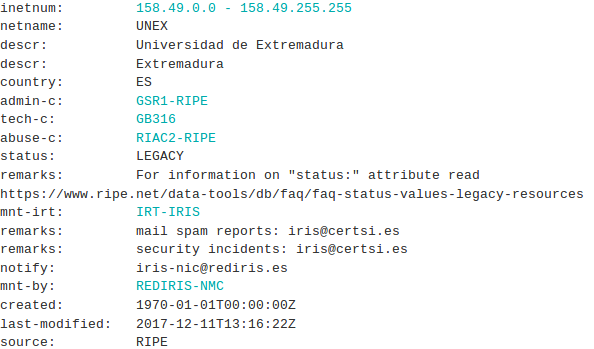
\includegraphics[scale=0.5]{pictures/data/ripedata.png}
	    	\caption{Datos obtenidos mediante RIPE}
   		\label{fig:Datos obtenidos mediante RIPE}
	\end{center}
\end{figure}
Se puede 
\subsection{Análisis de los gestos del ratón}
Este tipo de captura y análisis está centrado en el movimiento que hace el usuario a lo largo de la pantallla y los clicks realizados con el ratón sobre los diferentes enlaces que componen la interfaz. 
\newline \newline
Normalmente, la información que se obtiene por este método es útil tanto para desarrolladores, diseñadores y redactores de una página a la hora de evaluar el rendimiento, diseño y conocer los contenidos más relevantes, respectivamente. Esta técnica es tremendamente útil puesto que permite conocer cómo se \textit{mueven} los usuarios dentro de un sitio, que secciones dentro de una página visitan más, incluso generar mapas de calor con las zonas por las que más se mueven los usuarios y detectar así puntos calientes a los que prestar más atención, así como fugas de interés, encontrando puntos ciegos, para proceder a un análisis de las causas y mejorar así el rendimiento de un portal. 
\newline \newline
Desde un punto de vista técnico, esta recolección de datos puede ocurrir en tiempo real o bien los datos serán almacenados para manipularlos después. A día de hoy muchas \textit{suites} analíticas implementan esta funcionalidad a través de código Javascript insertado en las páginas con métodos que capturan y rastrean la interacción del ratón dentro de la página. 
\newline \newline
Este método a ido evolucionando con el tiempo hacia nuevas aproximaciones, como la predicción del click, donde mediante un programa que siga el movimiento del ojo del usuario y midiendo la dilatación de su pupila podemos predecir donde se realizará la pulsación y adaptar así la respuesta del servicio a la nueva situación prevista \cite{guachos}. 
\subsection{Cookies}
Las cookies, aunque estén tan de moda últimamente con la salida del \textit{nuevo} RGPD \cite{rgpd} (Reglamento General de Protección de Datos) sustituyendo a la nacional LOPD (Ley Oficial de Protección de Datos), surgieron en los albores de internet, siendo el primer método de \textit{rastreo} utilizado. 
\newline \newline 
Las cookies surgieron por la necesidad de mantener información sobre la sesión del usuario después de un login, mantener los elementos de un carrito de la compra o sencillamente para guardar información sobre preferencias del sitio (idioma, tema...). 
\newline \newline 
Estas cookies consisten en un par clave-valor que, generado por el servidor, es enviado al cliente para que este lo almacene en local. Más tarde esta información es consultada para adaptar el contenido en base a esa información.  
\newline \newline
En teoría, una cookie solo puede ser consultada por su origen, es decir, por el servidor que la generó, pero con el tiempo y la aparición de servidores compartidos (servidores de publicidad, por ejemplo) es posible generar una cookie que podrá ser consultada por todas las páginas que empleen ese servidor, estas son las llamadas \textit{third party cookies}, que guardan o usan información del usuario sin que este tenga que navegar directamente en su dominio, dado que está incrustada en la web anfitrión. 
\newline \newline 
Entre la información que es posible capturar con una cookie se incluye el sistema operativo, la dirección IP, el navegador, la ubicación, uso horario, idioma y lo más importante, los sitios por los que se navega. Por ejemplo, si se busca en una tienda online (pongamos Amazon como ejemplo), esa información sobre la búsqueda se queda almacenada en la cookie. Si otra web emplea publicidad de esa tienda, sabrá los términos de la búsqueda y podrá mostrar publicidad relacionada. 
\newline \newline 
Normalmente, la técnica para el rastreo con cookies pasa por la creación de un identificador único de usuario para asociarlo a la misma. Este ID nos mantendrá identificados durante nuestra navegación y será empleado por las páginas que usen los servicios del proveedor de esa cookie. De esta manera, si cada página emplea cookies propias o de terceros, seremos conscientes de que estamos continuamente generando información y que además esta información no pasa desapercibida, si no que es registrada, enviada, usada y compartida entre compañías. 
\section{Google y la plataforma Android}
Hasta ahora hemos visto los métodos de captura de información a través de la web, pero en los últimos 10 años el mercado ha cambiado mucho con la aparición del smartphone. Las cifras son apabullantes, en 2008 nace Android y en el tramo de 10 años la implantación del smartphone en la sociedad está fuera de cualquier duda. 
\begin{figure}[H]
	\begin{center}
   		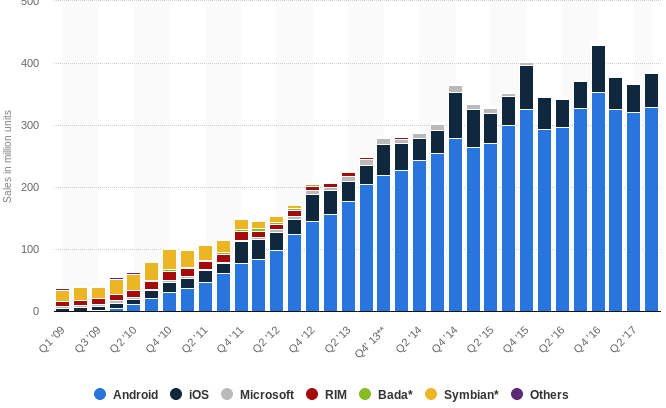
\includegraphics[scale=0.5]{pictures/data/smartphone_sells.png}
	    	\caption{Venta global de smarthpones según el sistema operativo}
   		\label{fig:Venta de Smartphones}
	\end{center}
\end{figure}
Es por tanto una línea muy a tener en cuenta, estamos hablando que llevamos un dispositivo inteligente con nosotros todo el día, se ha convertido en una extensión más de nuestro cuerpo. Un pedazo de tecnología que nos permite estar conectados 24 horas al día, sin interrupción. 
\newline \newline
Pensar que aún teniendo eso en el bolsillo aún somos anónimos es pecar de insensatos, cuanta más conexión mayor control. Las grandes compañías, en su afán por conocer a sus usuarios, no desaprovechan este hecho, aunque a nosotros muchas veces se nos pase por alto. Llevamos en nuestro bolsillo un aparato que no deja de ser un ordenador miniaturizado, que nos permite comunicarnos con nuestros contactos, acceder a Internet y usar servicios que nos hacen la vida más fácil. Pero no se paga nada, a parte del coste del propio dispositivo físico. 
\newline \newline
Recordemos entonces las palabras citadas al inicio del trabajo, cuando no pagas por un producto es porque el producto eres tú. Consumimos tecnología mientras que la tecnología nos consume a nosotros, usamos teléfonos cuyo código fuente sólo es accesible para los creadores del mismo, no sabemos que llevamos encima, en el bolsillo, un aparato que expande nuestras capacidades de comunicación como nunca antes ha sucedido en la historia de la humanidad. 
\newline \newline
Personalmente, creo que esto debería y que realmente está empezando a cambiar, si el teléfono es una parte más de nuestro cuerpo (algo incuestionable), deberíamos aplicar el mismo celo que al resto de cuestiones de nuestra vida. Del mismo modo que no consumimos determinados productos (por ejemplo, gente que evita los transgénicos, carnes rojas, etc) deberíamos comenzar a plantearnos el origen de ese \textit{cacharro} que llevamos todo el día en nuestro bolsillo, con el que compartimos nuestra intimidad y usamos para hablar con amistades y seres queridos. 
\newline \newline
En el caso que nos atañe, Android, viene de la mano de Google, empresa que vive (entre otras cosas) del \textit{segmentation-targeting}. Quieren nuestros datos y nosotros se los damos sin pestañear. Incluso siendo conscientes de que nuestras costumbres están siendo analizadas, perfiladas y almacenadas dentro de un modelo, no dejamos de consumir sus servicios. 
\newline \newline
Esa esclavitud tácita está con nosotros desde que abrazamos la tecnología, cada vez más conectados, cada vez más esclavos. Por ello, es bueno mirar con ojos críticos a las compañías a las que entregamos nuestras vidas (la vida digital y real están tan mezcladas que hacer distinciones es absurdo) y pararnos a pensar que sucede realmente con nosotros, los consumidores. ¿Realmente no estamos pagando nada por los servicios que se nos ofrecen? ¿Deberían pagarnos ellos a nosotros por invadir nuestra privacidad? ¿Asumimos el coste que conllevan las facilidades que este modelo de consumo tecnológico nos ha impuesto?. 
\newline \newline
Veamos cuánto de verdad hay en estas palabras y si realmente existen casos documentados de que esto esté sucediendo así. 
\subsection{Los servicios de Google y la localización}
Durante el 2017 salió a la luz la noticia de que Google registraba y almacenaba la localización de los teléfonos Android incluso cuando este servicio estaba desactivado \cite{googleLocalizacion}. Esto fue confirmado poco después por Google, quien afirmó que abandonaron esa práctica al poco de darse a conocer estos hechos. 
\newline \newline 
Es lógico pensar que cuando estamos usando algún servicio de google que incluya localización esta se mande a sus servidores, son sus reglas y si quieres usar el servicio es un coste asumido. De hecho, Google no oculta esta práctica, pudiendo consultar tu histórico de localizaciones en su propio portal \cite{googleLocationHistory}. A continuación se adjunta la imagen del histórico de localizaciones del autor en la ciudad de Cáceres. 
% IMAGEN 
\begin{figure}[H]
\begin{center}
	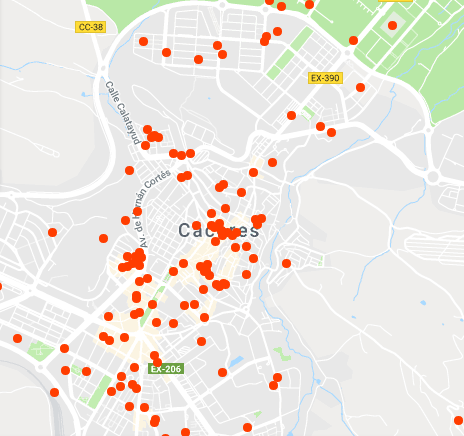
\includegraphics[scale=0.5]{pictures/data/google_location_history.png}
	\caption{Historial de localizaciones en Cáceres}
	\label{fig:Historico de localizaciones}
\end{center}
\end{figure}
Por lo tanto, esta práctica de Google no es ningún secreto, siendo además una \textit{feature} de su sistema y sus servicio de mapas, ofreciendo rutas alternativas al itinerario habitual en función del tráfico, guardar la posición del aparcamiento, etc. 
\newline \newline 
El problema viene cuando se pierde el control de esta información. La  noticia citada al principio de esta sección pone en relieve la problemática, puesto que Google envía información de tu localización a sus servidores incluso cuando este servicio está desactivado en el teléfono y la SIM quitada. 
\newline \newline 
Pero, ¿cómo sabe Google donde estás si tienes este servicio desactivado? Aprovecha las antenas de telefonía. En primer lugar se identifica al usuario por su CellID (identificador único de cada teléfono) y cada vez que el terminal se conecta a una torre se manda la información de esa conexión junto con el cellID a sus servidores. Esa información de la conexión incluye el identificador de la torre, que permite saber su localización exacta. 
\newline \newline 
En un primer momento pudiera parecer que esta práctica no es demasiado intrusiva, solamente se manda información sobre la torre más cercana a la que se ha conectado el teléfono, pero cuando esta práctica se extiende a lo largo del tiempo (durante 24 horas por ejemplo), se puede llegar a triangular la posición exacta del teléfono gracias a la información de las torres a las que se ha ido conectando. 
\newline \newline 
Google reconoció los hechos y aportó más información al respecto, afirmando que además de la información de las torres de telefonía empleaban otros datos, como la cercanía con redes Wifi u otros dispositivos. 
\newline \newline 
Esto hila con otro escándalo que esta vez esta relacionado con el coche que Google emplea para mapear las ciudades para su servicio de Google Maps. Resulta que este coche, además de fotografiar las calles, iba recolectando la información de las redes Wifi abiertas, obteniendo así un mapeo de las redes y su localización exacta \cite{gmaps}. 
\newline \newline
Con estas fuentes de datos es tremendamente sencillo para Google saber que está haciendo el usuario en cada momento, puesto que es posible determinar si estás en un núcleo urbano, en lo alto de una montaña, si vas andando, bicicleta, usas el transporte público, etc. Esta información es tremendamente útil para hacer crecer la base de conocimiento de Google y mejorar el targeting de su servicio de publicidad (AdWords). 
\subsection{Aplicaciones de terceros}
Hemos visto como Google aprovecha su propia plataforma para registrar datos del usuario, veamos ahora como otras compañías se aprovechan de ella para recolectar información de los usuarios a través de las aplicaciones que implementan para este mismo sistema. 
\subsubsection{Aplicación de La Liga}
A principios de Junio de 2018 salió a la luz un nuevo caso de espionaje al usuario. En esta ocasión se trataba de la aplicación oficial de La Liga \cite{noticiaLaLiga}, la cual usaba el micrófono de los usuarios para, en teoría, detectar posibles fraudes. 
\newline \newline 
Para ello la aplicación pedía permisos de micrófono y de localización para, de nuevo supuestamente, activar esta funcionalidad en las franjas horarias de los partidos de fútbol y analizando el audio capturado junto con la localización, detectar posibles fraudes. 
\newline \newline 
El revuelo vino porque los usuarios no eran conscientes de que esto sucediese, lo cual dice muy poco de nosotros como usuarios, se estaban aceptando unas condiciones legales en las figuraba una línea indicando claramente este uso, así como la autorización explícita a la aplicación para usar el micrófono. 
\newline \newline 
Al poco tiempo de que la noticia salía a la luz la empresa realizó un comunicado donde se repetían lo dicho arriba, que ese audio era únicamente para detectar fraudes en el territorio Español y no era usado para otros propósitos. Dada la vaguedad de las declaraciones, hubo usuarios que analizaron la aplicación y estudiaron su comportamiento \cite{laLigaJaker}, lo que nos permite hacer un resumen de como está implementada esta lógica. 
\newline \newline 
En primer lugar, la aplicación comprobaba los permisos de micrófono y localización en cada ejecución, solicitándolos en caso de no estar asignados. Después, mediante un listener, detecta cada cambio de ubicación y va creando un registro que, cada 30 minutos, se manda a un servidor y se borra del teléfono. 
\newline \newline 
El micrófono, en cuanto está disponible, comienza a grabar y mandar los archivos al servidor. Durante cuanto tiempo permanece activa esa grabación es un misterio, así como el comportamiento de la activación del micrófono, puesto que lo lógico sería pensar que la aplicación, en función de la localización y el horario, active el micrófono, pero el análisis del código rebela que esta activación es arbitraria y nada tiene que ver con cuándo suceden los partidos de fútbol 
\newline \newline 
Esto ha demostrado que la escucha a los usuarios por parte de las compañías es una práctica que está a la orden del día, de hecho, cada vez son más las voces que afirman que Facebook a través de su aplicación emplea el micrófono para escuchar conversaciones privadas y aunque Facebook ha negado siempre esta práctica, las sospechas siempre estarán ahí, quedando demostrado además, como acabamos de ver, que ésta práctica existe y lo preocupante realmente es saber que pasa con ese archivo de audio desde el momento en el que sale del teléfono, puesto que se pierde cualquier control sobre estos datos. 
\subsubsection{Aplicación Linterna}
En este caso, vamos a irnos a una aplicación que saltó a la palestra a lo largo de 2013, cuando se descubrió que una aplicación a primera vista inocente dedicada a activar el led de la cámara y proveer así de una linterna, mandaba los datos de ubicación de sus usuarios a sus servidores junto con datos acerca de las redes wifi disponibles para más tarde vender los datos a terceros. 
\newline \newline 
Este caso está ampliamente documentado, llegando a publicar un comunicado de la Comisión Federal del Comercio de EEUU (un homólogo al patrio FACUA) donde se describen y condena esta práctica \cite{CFCEEUU}. 
\newline \newline 
En el documento citado se condena a la compañía por estas acciones, entre las que se incluyen la posibilidad de tomar fotos a través de la cámara del dispositivo sin que el usuario tome partido en ello y el envío de datos de localización a empresas de publicidad. 
\newline \newline 
Este caso nos sirve como muestra, junto con el anterior, de que estas prácticas llevan muchos años en el sector y pone en relieve la falta de control de los datos del usuario, además, nos hace plantearnos que hacen las grandes compañías con sus aplicaciones, en las que entra en juego mayor alcance de usuarios y por tanto mayor rédito económico. 
\section{Dispositivos IOT}
En los últimos años hemos visto como \textit{el internet de las cosas} ha comenzado a implantarse en los hogares, desde bombillas inteligentes que podemos controlar con nuestro teléfono hasta frigoríficos que nos avisan cuando falta algún producto en la nevera. 
\newline \newline 
Esta evolución ha seguido su camino y las compañías no han querido perderse la fiesta, desarrollando cada una sus propias versiones de asistentes personales para, en teoría, facilitarnos la vida dentro de nuestra casa, es el caso del Google Home de Google, Alexa de Amazon o el Apple homePod de Apple. Estos dispositivos comparten todos la característica de  activarse mediante comandos de voz, lo cual implica una escucha pasiva en segundo plano a la espera de reconocer algún comando y activarse. 
\newline \newline 
Esta tecnología, dado su enorme potencial, hizo que muchos usuarios mirasen con lupa a estos dispositivos, dando como resultado lo que veremos a continuación. 
\subsection{Asistentes personales}
En este último año han irrumpido en el mercado los asistentes personales, introducidos por Google, Amazon y Apple. Estos asistentes son precisamente eso, un asistente personal que nos ayuda a gestionar nuestra agenda, consultar Internet e interactuar con el ecosistema de cada compañía. 
\newline
\newline
Todos comparten la misma funcionalidad básica, incorporan un micrófono que permanece siempre activo esperando a recibir el comando de activación. Normalmente este comando es una palabra clave que permite que el dispositivo se active, Ok Google! en el caso del Google Home, Alexxa… en del Amazon Echo, etc. Una vez el dispositivo está activo pasa a un estado de escucha activa donde atiende las consultas del usuario a través de la voz. 
\newline
\newline
No hay duda de que se tratan de aparatos tremendamente interesante y que a día de hoy es hacia donde se dirige el mercado, Meter en casa un dispositivo con inteligencia artificial que nos facilite la vida, podamos encender la televisión, reproducir música, hacer anotaciones, llamar a nuestros contactos, etc, gestionado únicamente por voz es un producto realmente atractivo.  
\newline
\newline
Pero como hemos estado viendo hasta ahora, las compañías quieren nuestros datos, meter en nuestros hogares dispositivos inteligentes que se encuentran siempre escuchando en segundo plano, a estas alturas, no parece una decisión muy prudente. 
\newline
\newline
Esto demuestra el afán de las compañías por descubrir más de sus usuarios, uno de los grandes escollos que tienen hasta el momento es que sólo capturan la información cuando el usuario interactúa con sus servicios, pero permanecen a ciegas el resto del tiempo. Si consiguen meter en los hogares estos aparatos, que permiten escuchar conversaciones privadas en cualquier momento, aumentará su capacidad de recolección de datos y por tanto mejorar infinitamente su \textit{targeting}, puesto que no sólo sabrán lo que hace el usuario cuando usa su aplicación, si no que les permitirá saber como se comporta durante su vida privada. 
\newline
\newline
En el caso de Amazon Alexa ha quedado demostrado que el dispositivo realiza escuchas aleatorias \cite{alexaSpy}, de duración indeterminada, que, hasta donde se ha podido averiguar, quedan almacenadas en el dispositivo. No es así en el caso del Google Home, donde todos los fragmentos de audio que se registren son enviados a sus servidores, de hecho lo dejan bien claro en su política de privacidad \cite{GooglePrivacy}
\newline
\newline
Esto demuestra el afán de estas empresas por conocer cada vez más detalles de sus usuarios, hasta el punto de perseguir el objetivo último de que todos los hogares cuenten con un dispositivo inteligente que les permita conocer los hábitos de sus usuarios en su vida privada. 
\newline
\newline
Este afán queda explicado cuando reparamos en el problema que llevamos denotando durante el desarrollo de estas páginas, la información recogida, hasta ahora, es parcial, sólo nos muestra al usuario cuando usa sus productos, el resto del tiempo permanece invisible para ellos. Si finalmente consiguen su objetivo (un dispositivo en cada casa) conseguirán saltar esa brecha y poder obtener un perfil completo del usuario, sabiendo que dice, hace y cómo se comporta a lo largo de las 24 horas del día, sin interrupción, los 365 días del año. 
\newline
\newline
Justo ese es el objetivo de este trabajo, lo cual nos indica que no vamos del todo mal encaminados. Cada vez es más importante conocer a nuestros usuarios, pero hasta ahora este conocimiento estaba limitado al producto en sí, si conseguimos extraer un perfil de comportamiento completo del mismo tendremos en nuestras manos una información con un enorme potencial, que nos permitirá abrir nuevas líneas de investigación, las cuales, en buenas manos, podrán cambiar para bien la vida de muchas personas. 
\newline
\newline
Nuestro objetivo final, y lo que se persigue con este proyecto, es que esta información no esté exclusivamente en manos de compañías que sólo quieren ver incrementados sus beneficios, si no que sea accesible para cualquier equipo de desarrollo que tenga buenas intenciones (en nuestro caso, el equipo del SpiLab de la Epcc). 
\newpage
\chapter{Requisitos del proyecto}
En esta capítulo se analiza el problema planteado por el proyecto y se detalla su descomposición como requisitos de un sistema software. No hay que perder de vista que nuestro objetivo final será monitorizar las aplicaciones del usuario y registrar información acerca de cómo éste interactúa con el medio.
\newpage
\section{Requisitos}
Se propone el desarrollo de una aplicación móvil que, en segundo plano, registre los movimientos del usuario y la interacción que realiza con el teléfono. Este registro de actividad debe cubrir los requisitos listados a continuación para componer un sistema final que satisfaga los objetivos expuestos con anterioridad. 
\subsection{Requisitos funcionales}
El sistema deberá: 
\begin{itemize}
  \item Registrar cada aplicación que lanza el usuario detectando y almacenando el nombre del paquete asociado a ella. 
  \item Aportar un contexto temporal de cuando las aplicaciones son ejecutadas, esto es, el \textit{timestamp} del momento de su ejecución. 
  \item Incluyendo lo anterior, registrar el uso dado a aplicaciones relacionadas con, comunicación, mensajería instantánea, búsqueda web,redes sociales y por último sensores. 
  \item Dentro de comunicación se incluye la aplicación de Gmail, Mensajes (sms) y el Teléfono. 
  \item Dentro mensajería instantánea prestaremos atención a Telegram, Whatsapp Messenger y Facebook Messenger. 
  \item Como aplicaciones relacionadas con la búsqueda en la web estarán la Chrome Browser y Google Search. 
  \item En las aplicaciones de redes sociales; Twitter, Facebook e Instagram.
  \item Los sensores que escucharemos serán el emisor de GPS, acelerómetro, presión, giroscopio y temperatura.
\subsubsection{Aplicaciones de comunicación}
  \item En  \textbf{Gmail} capturar, la dirección de correo del emisor. 
  \item La dirección de correo del receptor(es). 
  \item El asunto del correo electrónico. 
  \item El contenido, cuerpo de dicho correo. 
  \item En \textbf{Mensajes} se deberá capturar, el destinatario. 
  \item El cuerpo del mensaje. 
  \item En \textbf{Teléfono} se deberá capturar, el destinatario de la llamada. 
  \item Tiempo total invertido en ella. 
\subsubsection{Aplicaciones de mensajería instantánea}
  \item En \textbf{Telegram} capturar, el nombre del contacto o grupo interlocutor. 
  \item Los mensajes enviados en la conversación por parte del usuario. 
  \item En \textbf{Whatsapp} capturar, el nombre del contacto o grupo interlocutor. 
  \item Los mensajes enviados en la conversación por parte del usuario. 
  \item En \textbf{Facebook Messenger} capturar, el nombre del contacto o grupo interlocutor. 
  \item Los mensajes enviados en la conversación por parte del usuario. 
\subsubsection{Aplicaciones de búsqueda en la web}
  \item En \textbf{Chrome} capturar las páginas visitadas. 
  \item El tiempo invertido en cada una de ellas. 
  \item En \textbf{Firefox} capturar las páginas visitadas. 
  \item El tiempo invertido en cada una de ellas. 
  \item En \textbf{Búsqueda de Google} el objeto de búsqueda. 
\subsubsection{Aplicaciones de redes sociales}
  \item En \textbf{Twitter} capturar, el nombre de los perfiles visitados. 
  \item Los tuits publicados. 
  \item El contenido de los mensajes directos. 
  \item En \textbf{Facebook} capturar, el nombre de los perfiles visitados. 
  \item Los comentarios hechos en dichos perfiles. 
  \item Los estados compartidos dentro de la red social. 
  \item Las subidas de fotos y su título. 
\end{itemize}
\subsubsection{Sensores}
\begin{itemize}
  \item Del sensor relacionado con la ubicación \textbf{GPS} deberemos registrar cada cambio de coordenadas que registre el teléfono. 
  \item Mediante el \textbf{acelerómetro} registraremos los cambios en la aceleración del teléfono. 
  \item Con el sensor de \textbf{presión} registraremos los cambios de altitud del teléfono. 
  \item Con el \textbf{giroscopio} para detectar y registrar  los movimientos que realiza el teléfonpo. 
  \item El sensor de \textbf{temperatura} nos permitirá registrar, como no, la temperatura ambiente del dispositivo. 
\end{itemize}
\newpage
\subsection{Requisitos no funcionales}
\begin{itemize}
	\item Versión. El sistema deberá soportar una versión limpia de Android 8.0. 
	\item Eficiencia. Dado que el sistema debe registrar en tiempo real toda la información generada por el usuario, deberá ser capaz de capturarla en tiempo real, al mismo tiempo que se analiza y almacena. 
	\item Privacidad. El usuario deberá autorizar explícitamente al software desarrollado permisos de accesibilidad, de modo que sea consciente de que existe una aplicación monitorizando parte de su actividad.
	\item Robustez. Debido a que el sistema debe estar constantemente capturando, el software debe ser tolerante a fallos y mantener el servicio siempre disponible.  
	\item Seguridad. La base de datos local deberá estar protegida ante el acceso indebido a los datos. 
\end{itemize}
Los requisitos listados en este capítulo tienen como objetivo definir la implementación de un sistema que permita, en última instancia, obtener un perfil completo del usuario. 
\newline \newline 
Por un lado, los requisitos funcionales nos guiarán en la captura de información del usuario. Como se ha visto, tenemos 5 grandes grupos, que nos permiten conocer todas las facetas de la vida de este, ó, al menos, todas las que pasen por usar el terminal. 
\newline \newline
Por un lado la comunicación, escuchando aplicaciones como Gmail, el envío de sms y las llamadas telefónicas. Con la mensajería instantánea cubrimos las tres grandes aplicaciones en este campo, Whatsapp, Telegram y Facebook Messenger. En la navegación web, otra de las grandes tareas que hacemos con nuestros teléfonos, escucharemos Chrome, Firefox y la barra de Búsqueda Rápida de Google. 
\newline \newline 
También podremos saber como interactúa el usuario con sus contactos a través de las redes sociales, puesto que almacenaremos datos provenientes de Facebook y Twitter. Y por último, para conocer cómo interactúa el usuario con el medio físico, recolectaremos los datos de los sensores físicos que incorporan la mayoría de terminales. 
\newline \newline 
Todos estos requisitos, junto con los no funcionales, cuyo objetivo es aportarle robustez al proyecto, nos permitirán desarrollar un sistema completo que abarque los usos mayoritarios del teléfono, obteniendo así un perfil completo de cómo un usuario interactúa y se relaciona con su terminal y entorno. 
\break

\chapter{Análisis}
Para centrar el problema y enfocar los requisitos a un proceso que nos lleve a obtener un proyecto de ingeniería, haremos uso de distintos diagramas que nos ayudaran a resolver el problema y plantear una solución. Así en el capítulo nos encontramos con los diagramas de casos de uso, indicando las tareas que debe resolver el sistema, y un diagrama de arquitectura a alto nivel que plantea una solución inicial. 
\pagebreak
\section{Diagramas de Casos de Uso}
Los casos de uso del sistema están planteados de modo que el usuario, al interactuar con el teléfono, dispara siempre la acción, aunque en muchos casos la acción del usuario será pasiva, es decir, no tendrá que realizar ninguna acción en concreto para disparar, por ejemplo, la captura de los sensores, pero será su propia actividad la que nos permita realizar dicha captura. 
\newline
\newline
Por lo demás, hemos agrupado las aplicaciones en 5 categorías, comunicación, mensajería, navegación web, redes sociales y sensores. Dado que la mayoría de estas aplicaciones comparten la información a capturar, los veremos agrupados por comodidad para el lector. 
%%% ------ 
\begin{figure}[H]
	\begin{center}
		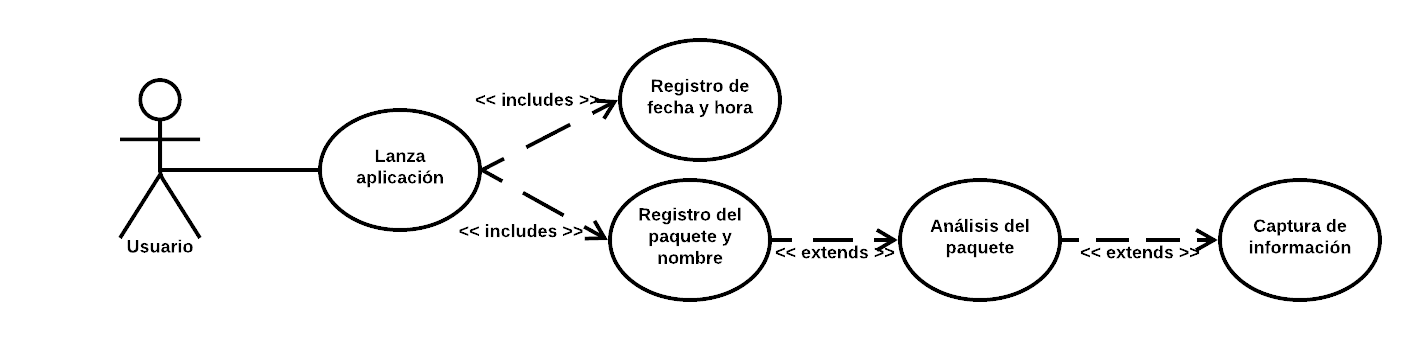
\includegraphics[scale=0.7]{pictures/usecases/usecases01.png} % include ./img/imagen.[pdf|png|jgp] si es pdflatex o ./img/imagen.eps si es latex
	\end{center}
	\caption[Casos de uso 01]{Casos de uso de cualquier aplicación.}
\end{figure}
%%% ------
Vemos como la captura de información extiende del lanzamiento de una aplicación, esto es así porque esta captura no se hará siempre, si no que dependerá de si la aplicación lanzada es objeto de captura. 
\pagebreak
Si nos centramos en el apartado de aplicaciones de comunicación; 
%%% ------ 
\begin{figure}[H]
	\begin{center}
		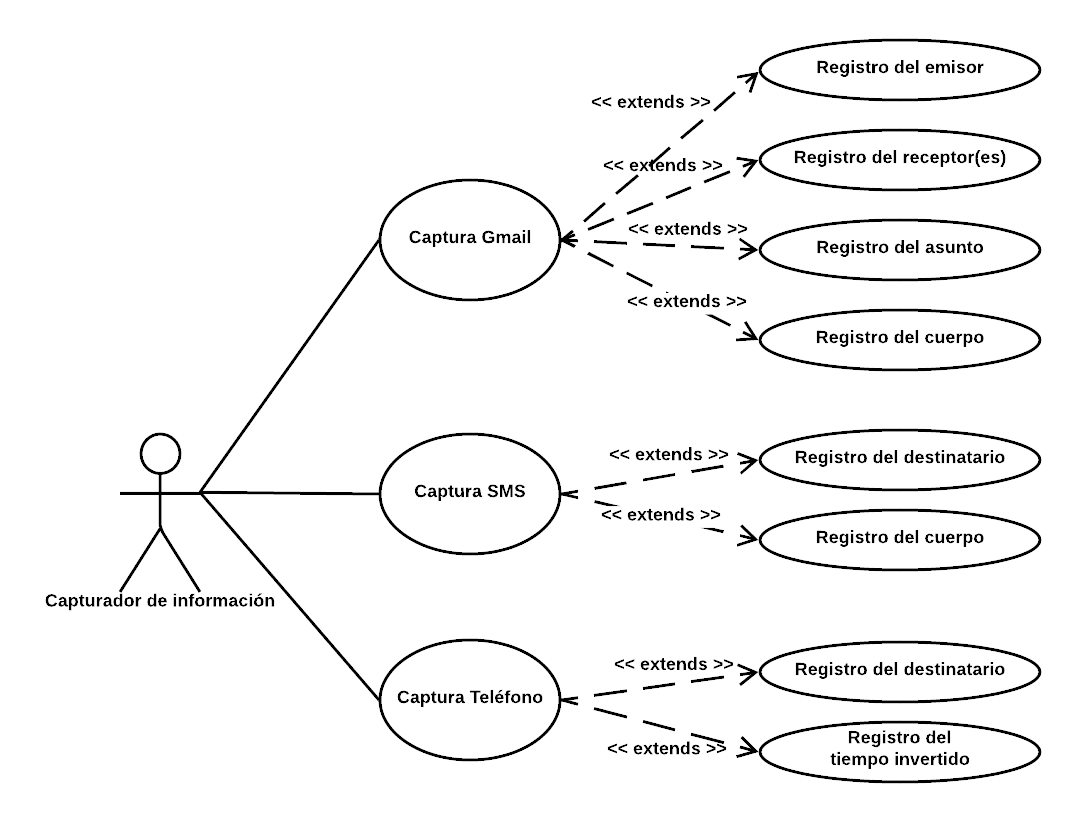
\includegraphics[scale=0.70]{pictures/usecases/usecases02.png} % include ./img/imagen.[pdf|png|jgp] si es pdflatex o ./img/imagen.eps si es latex
	\end{center}
	\caption[Casos de uso 02]{Casos de uso de aplicaciones de comunicación.}
\end{figure}
%%% ------
En el grupo de mensajería instantánea.
%%% ------ 
\begin{figure}[H]
	\begin{center}
		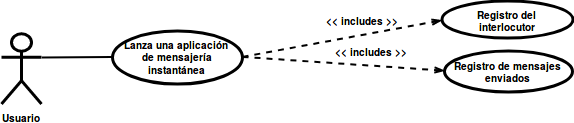
\includegraphics[scale=0.70]{pictures/usecases/usecases03.png} % include ./img/imagen.[pdf|png|jgp] si es pdflatex o ./img/imagen.eps si es latex
	\end{center}
	\caption[Casos de uso 03]{Casos de uso de aplicaciones de mensajería instantánea.}
\end{figure}
%%% ------
Aplicaciones de navegación y consulta de la web. 
%%% ------ 
\begin{figure}[H]
	\begin{center}
		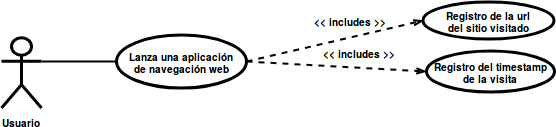
\includegraphics[scale=0.70]{pictures/usecases/usecases04.png} % include ./img/imagen.[pdf|png|jgp] si es pdflatex o ./img/imagen.eps si es latex
	\end{center}
	\caption[Casos de uso 04]{Casos de uso de aplicaciones de navegación web.}
\end{figure}
%%% ------
Si nos fijamos ahora en las aplicaciones de redes sociales, tenemos los siguientes casos de uso; 
%%% ------ 
\begin{figure}[H]
	\begin{center}
		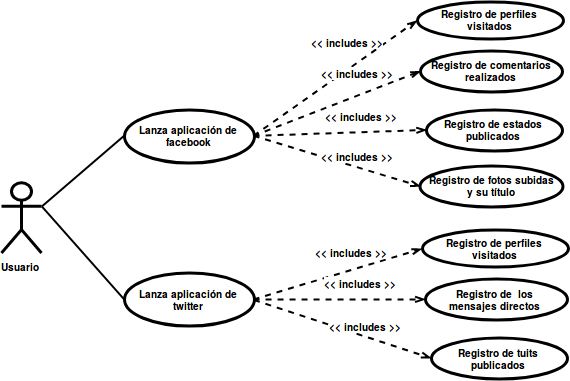
\includegraphics[scale=0.70]{pictures/usecases/usecases05.png} % include ./img/imagen.[pdf|png|jgp] si es pdflatex o ./img/imagen.eps si es latex
	\end{center}
	\caption[Casos de uso 05]{CU Apps RRSS.}
\end{figure}
%%% ------
Por último, en el apartado de los sensores, donde el actor será el capturador de la información de los sensores; 
%%% ------ 
\begin{figure}[H]
	\begin{center}
		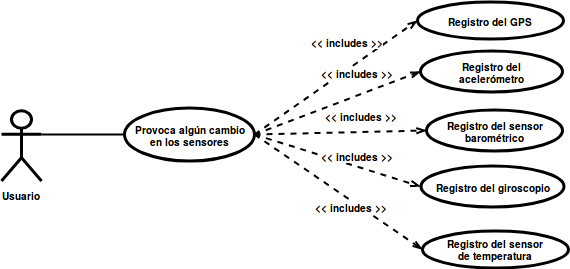
\includegraphics[scale=0.70]{pictures/usecases/usecases06.png} % include ./img/imagen.[pdf|png|jgp] si es pdflatex o ./img/imagen.eps si es latex
	\end{center}
	\caption[Casos de uso 06]{CU Sensores.}
\end{figure}
%%% ------
\pagebreak
\section{Arquitectura de alto nivel}
Teniendo claro cual es el propósito de nuestro sistema, debemos plantearnos cuáles serán los elementos que, interactuando entre ellos, resuelvan el problema final. 
\newline 
\newline
 
%----------- P A N O R A M I C O -------------------------------------------------

\begin{figure}[H]
  \begin{center}
     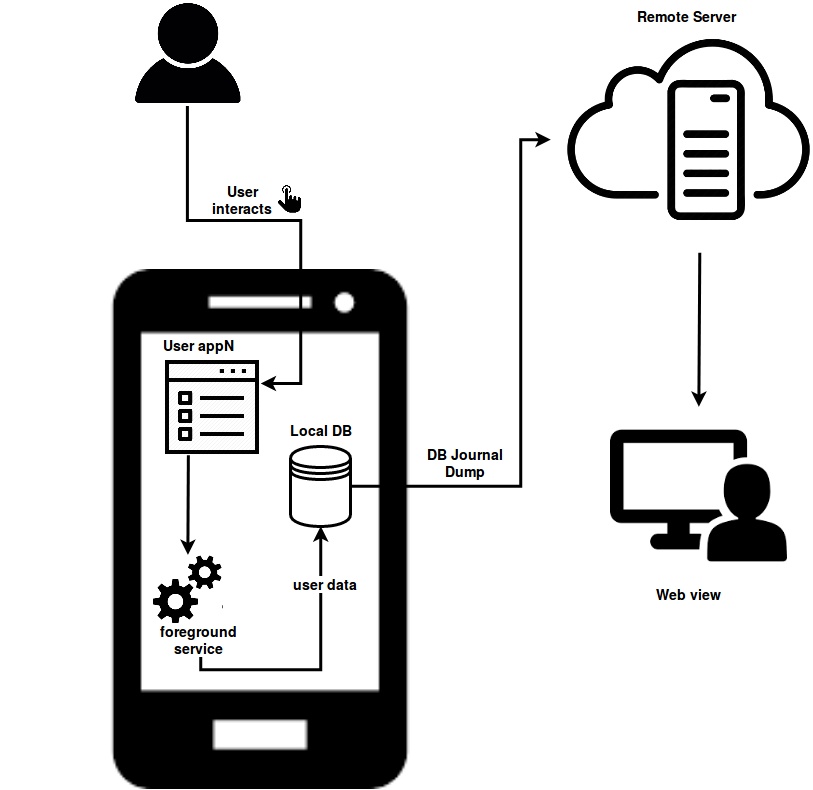
\includegraphics[width=0.8\textwidth]{pictures/architecture/highLevel/altonivel01.png}
  \end{center}
  \caption[Arquitectura de alto nivel]{Arquitectura de alto nivel.}
  \label{fig:LandscapeFigure}
\end{figure}
%----------- P A N O R A M I C O -------------------------------------------------

\newpage
Vemos que el sistema se compone gracias a tres componentes fundamentales, por un lado el usuario, fuente de nuestros datos, el propio teléfono, en donde capturaremos la información, y un servidor en la nube que recibirá de forma periódica los datos recogidos por el teléfono y que permitirá además consultarlos. 
\newline
\newline
\subsection{Smartphone}
Vayamos por partes pues y analicemos cada grupo de componentes. Por un lado el \textbf{smarthphone} y el \textbf{usuario}. Dado que el smartphone es la interfaz de acceso del usuario a las funciones del teléfono y sus aplicaciones, será entonces aquí donde centremos nuestro sistema y donde estarán la mayor parte de sus componentes, al menos todos los relacionados con la captura de información. 
\newline
\newline
Este proceso de captura se detalla en el siguiente fragmento de la arquitectura. 
 %%% ------ 
\begin{figure}[hbt]
  \begin{center} \setlength{\unitlength}{0.0105in}
     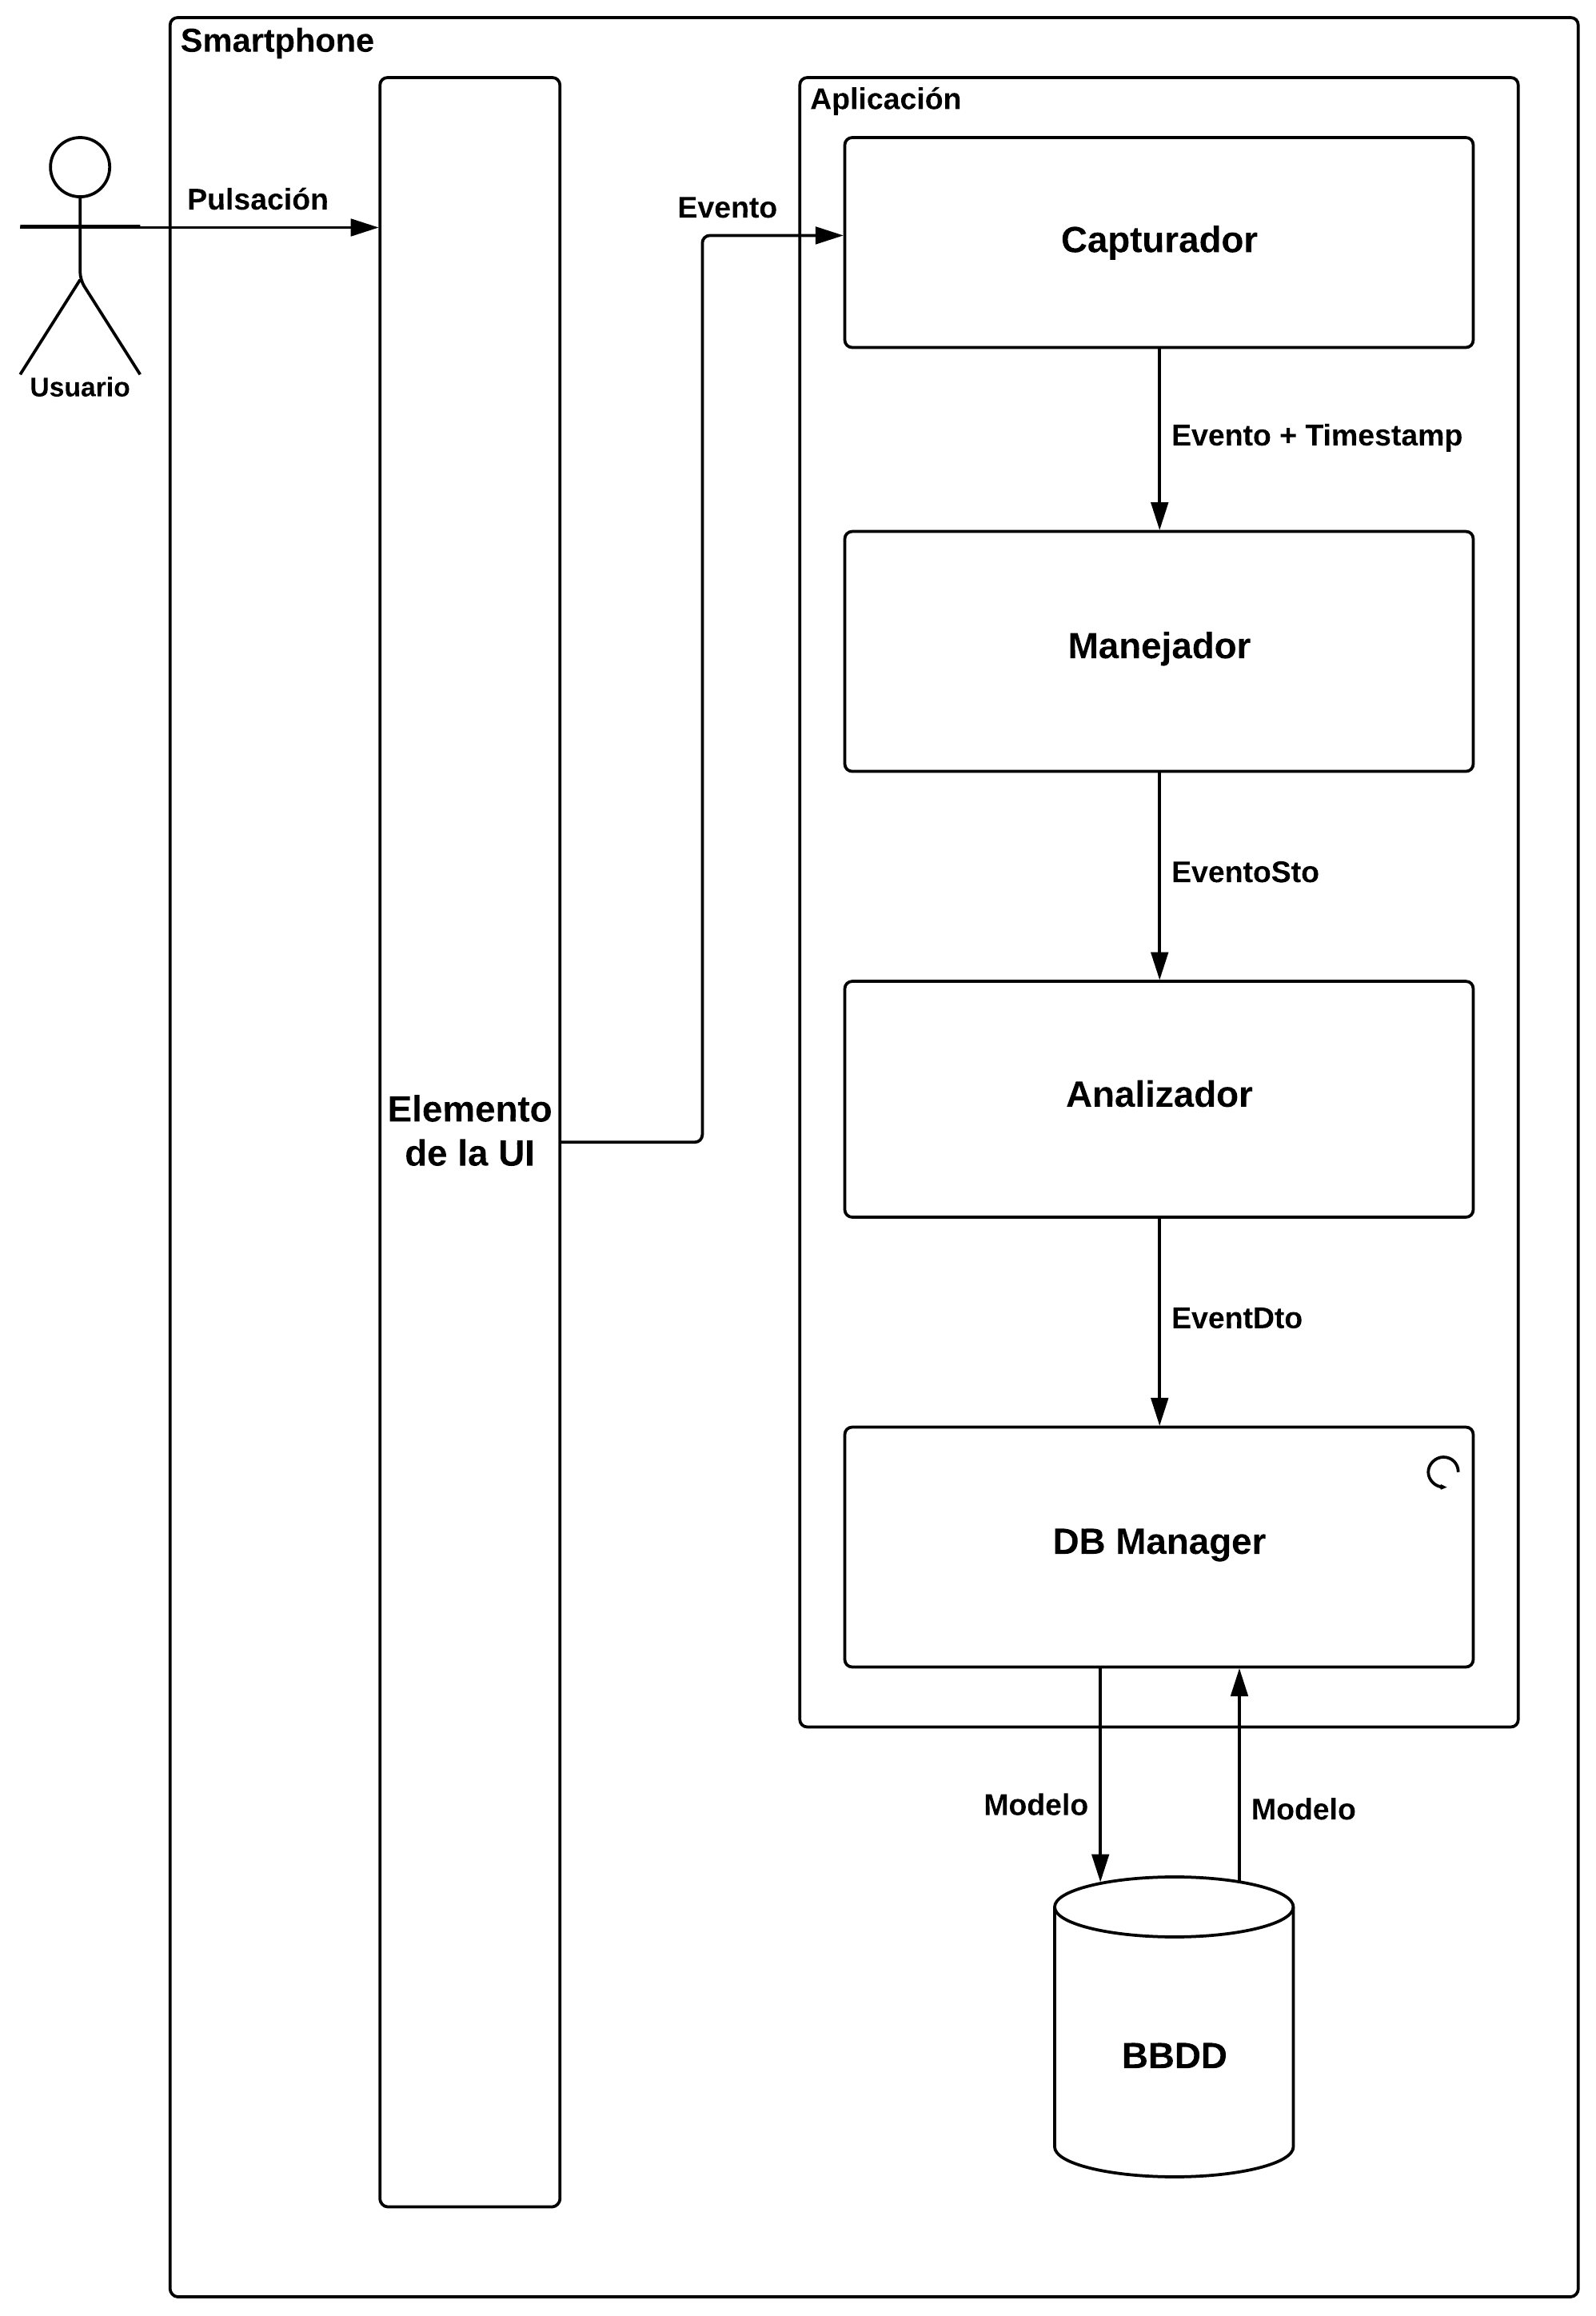
\includegraphics[width=0.6\textwidth]{pictures/architecture/highLevelArch02.png}
  \end{center}
  \caption[Arquitectura de alto nivel. Smartphone]{Arquitectura de alto nivel. Detalle de la parte móvil.}
\end{figure}
%%% ------
Toda la arquitectura parte del usuario, el cual interactúa con su teléfono mediante pulsaciones en la pantalla, que son recogidas por aplicaciones que le devuelven información al usuario mediante esa misma pantalla. Será entonces esta interfaz de usuario lo que nuestro sistema deberá escuchar y capturar. Por lo tanto tendremos una aplicación que recibirá las pulsaciones en los elementos de la interfaz del usuario (UI) bajo la forma de eventos. 
\newline
\newline
Vamos a desglosarla por cada elemento, viendo antes de cada componente la unidad de datos que va a manejar.
\newline
\newline
\subsubsection{Evento}
Estamos ante la información de entrada única y por tanto fundamental del sistema. Se trata de una unidad de datos compleja y sin estructurar. 
\newline
\newline
Los genera el sistema cada vez que ocurre un cambio notable en la pantalla, y su propósito es dar el mayor feedback posible del usuario. 
\newline
\newline
Muchas veces esta información no surge en el instante en el que se produce el evento, que no deja de ser una instantánea de la pantalla en ese momento, si no que se necesita un contexto. Esa es la parte complicada del desarrollo, necesitamos desarrollar sendas máquinas de estado 	que nos ayuden a relacionar los eventos entre ellos y procesarlos de tal modo que se produzca información útil y estructurada. 
\newline
\newline
Es por tanto, una unidad de datos muy cruda y desestructurada a la que hay que extraer el significado en su procesamiento en las capas inferiores. Por tanto este evento será producido por el sistema y la fuente de entrada del nuestro, a través del \textbf{capturador}.
\subsubsection{Capturador}
Se trata de un proceso que está siempre escuchando la aparición de nuevos eventos, con el objetivo de capturarlos y pasárselos al siguiente nivel de la arquitectura, el \textbf{manejador}. Su carga de trabajo realmente será poca, y consistirá en informar al manejador pasándole el evento junto al instante temporal en el que fué generado. 
\newline
\newline
Por lo tanto el capturador recibe eventos y genera eventos junto a su marca temporal para que los consuma el siguiente nivel, manejador. 
\subsubsection{Evento + timestamp}
No consiste en una unidad de datos como tal, puesto que sólo consiste en una fecha y hora y el propio evento asociado a ellos. 
\subsubsection{Manejador}
Recibe un evento y su marca horaria y debe encapsularlo para que el nivel inferior lo analice, es por tanto el nexo de unión entre los datos en bruto y los datos refinados. 
\newline
\newline
Para ello, cuando reciba el evento, en primer lugar lo encapsula junto a su marca horaria en un objeto que hemos llamado Sto. Simple Transfer Object. 
\newline
\newline
Una vez encapsulado, consulta la aplicación fuente del evento, es decir, la aplicación que lo generó, que nos permite establecer nuestro primer filtro y discernir si se trata de gmail, telegram, facebook... etc. 
\newline
\newline
En función de esto, se llamará a una implementación del analizador u otra, puesto que cada aplicación sigue su propio flujo lógico. Por ello se le comunica un Sto con la información fundamental que necesita. 
\subsubsection{Sto}
Es la unidad de datos empleado para comunicar el \textbf{manejador} con el \textbf{analizador}, se trata de una unidad de datos cuyo objetivo es encapsular la información en unidades contenidas y controladas. Será consumido por el analizador a través de la consulta de su evento y su marca horaria, siendo esta última fundamental para aportar el contexto necesario por el analizador. 
\subsubsection{Analizador}
Recibe los citados Stos, objetos sencillos, del manejador, para tratarlos, procesarlos y extraer su significao. 
\newline
\newline
Este procesamiento consisitirá en analizar, en base al modelo correspondiente, el patrón de llegada de los datos y en base a su contenido y el de eventos antecesores y sucesores, aportarle un contexto. Gracias a este modelo construiremos Dtos completos que representarán una unidad de información completa acerca del uso de la app.
\subsubsection{Dto}
Dtos, Data Transfer Objects, será la unidad última de información que genere nuestro sistema, representado así la información completa del usuario, es decir, uno de estos dtos contiene en su interior la interacción completa del usuario con cualquier servicio que le ofrezca el teléfono. 
\newline
\newline
Será por tanto contenido semántico de esta interacción, siendo por ejemplo, un dto una conversación mantenida por whatsapp con un contacto durante el intervalo de tiempo en el que estuvo activa, una búsqueda en el navegador... en resumen cualquier interacción, contextuada, del usuario con cualquiera de las apps que vamos a monitorizar. 
\newline
\newline 
Una vez estos Dtos están listos se les pasa al DB Manager. 
\subsubsection{DB Manager}
Capa encargada de la persistencia de los datos que le pasa el analizador. El manager los convierte en modelos para su almacenamiento en una base de datos local en la memoria del teléfono. 
\newline 
\newline 
En este manager recae una tarea también fundamental para el sistema, puesto que debe realizar un volcado periódico la base de datos a un servidor remoto para su seguridad y almacenamiento para posibles usos. Este funcionamiento de almacenar en local hasta que llegue el momento del volcado se ha tomado teniendo en mente la minimización del número de conexiones con el servicio externo. No podría ser una llamada a la API para persistir la información en la nube cada vez que una unidad de datos esté lista, puesto que la cantidad de información generada al día puede ser ingente. 
\newline \newline
La idea es almacenar en local hasta que pase un tiempo razonable (por ejemplo, 24 horas, tiempo en el que la base de datos se habrá ido llenando poco a poco) para volcar su contenido, liberar espacio y llevar los datos a la nube para persistir y asegurar la propia información. Así, no se satura la memoria interna del teléfono y la información viaja en bloques, minimizando la comunicación con el servicio externo y ahorrando batería, puesto que la conexión se realiza una vez al día. 
\newpage

\subsection{Servidor Remoto}
En este apartado analizaremos la arquitectura del entorno remoto planteado por la arquitectura. Consiste en un servicio en la nube que acepta el volcado que realiza la base de datos del teléfono cada poco tiempo y permite además visualizar los datos allí vertidos. 
 %%% ------ 
\begin{figure}[hbt]
  \begin{center} \setlength{\unitlength}{0.0105in}
     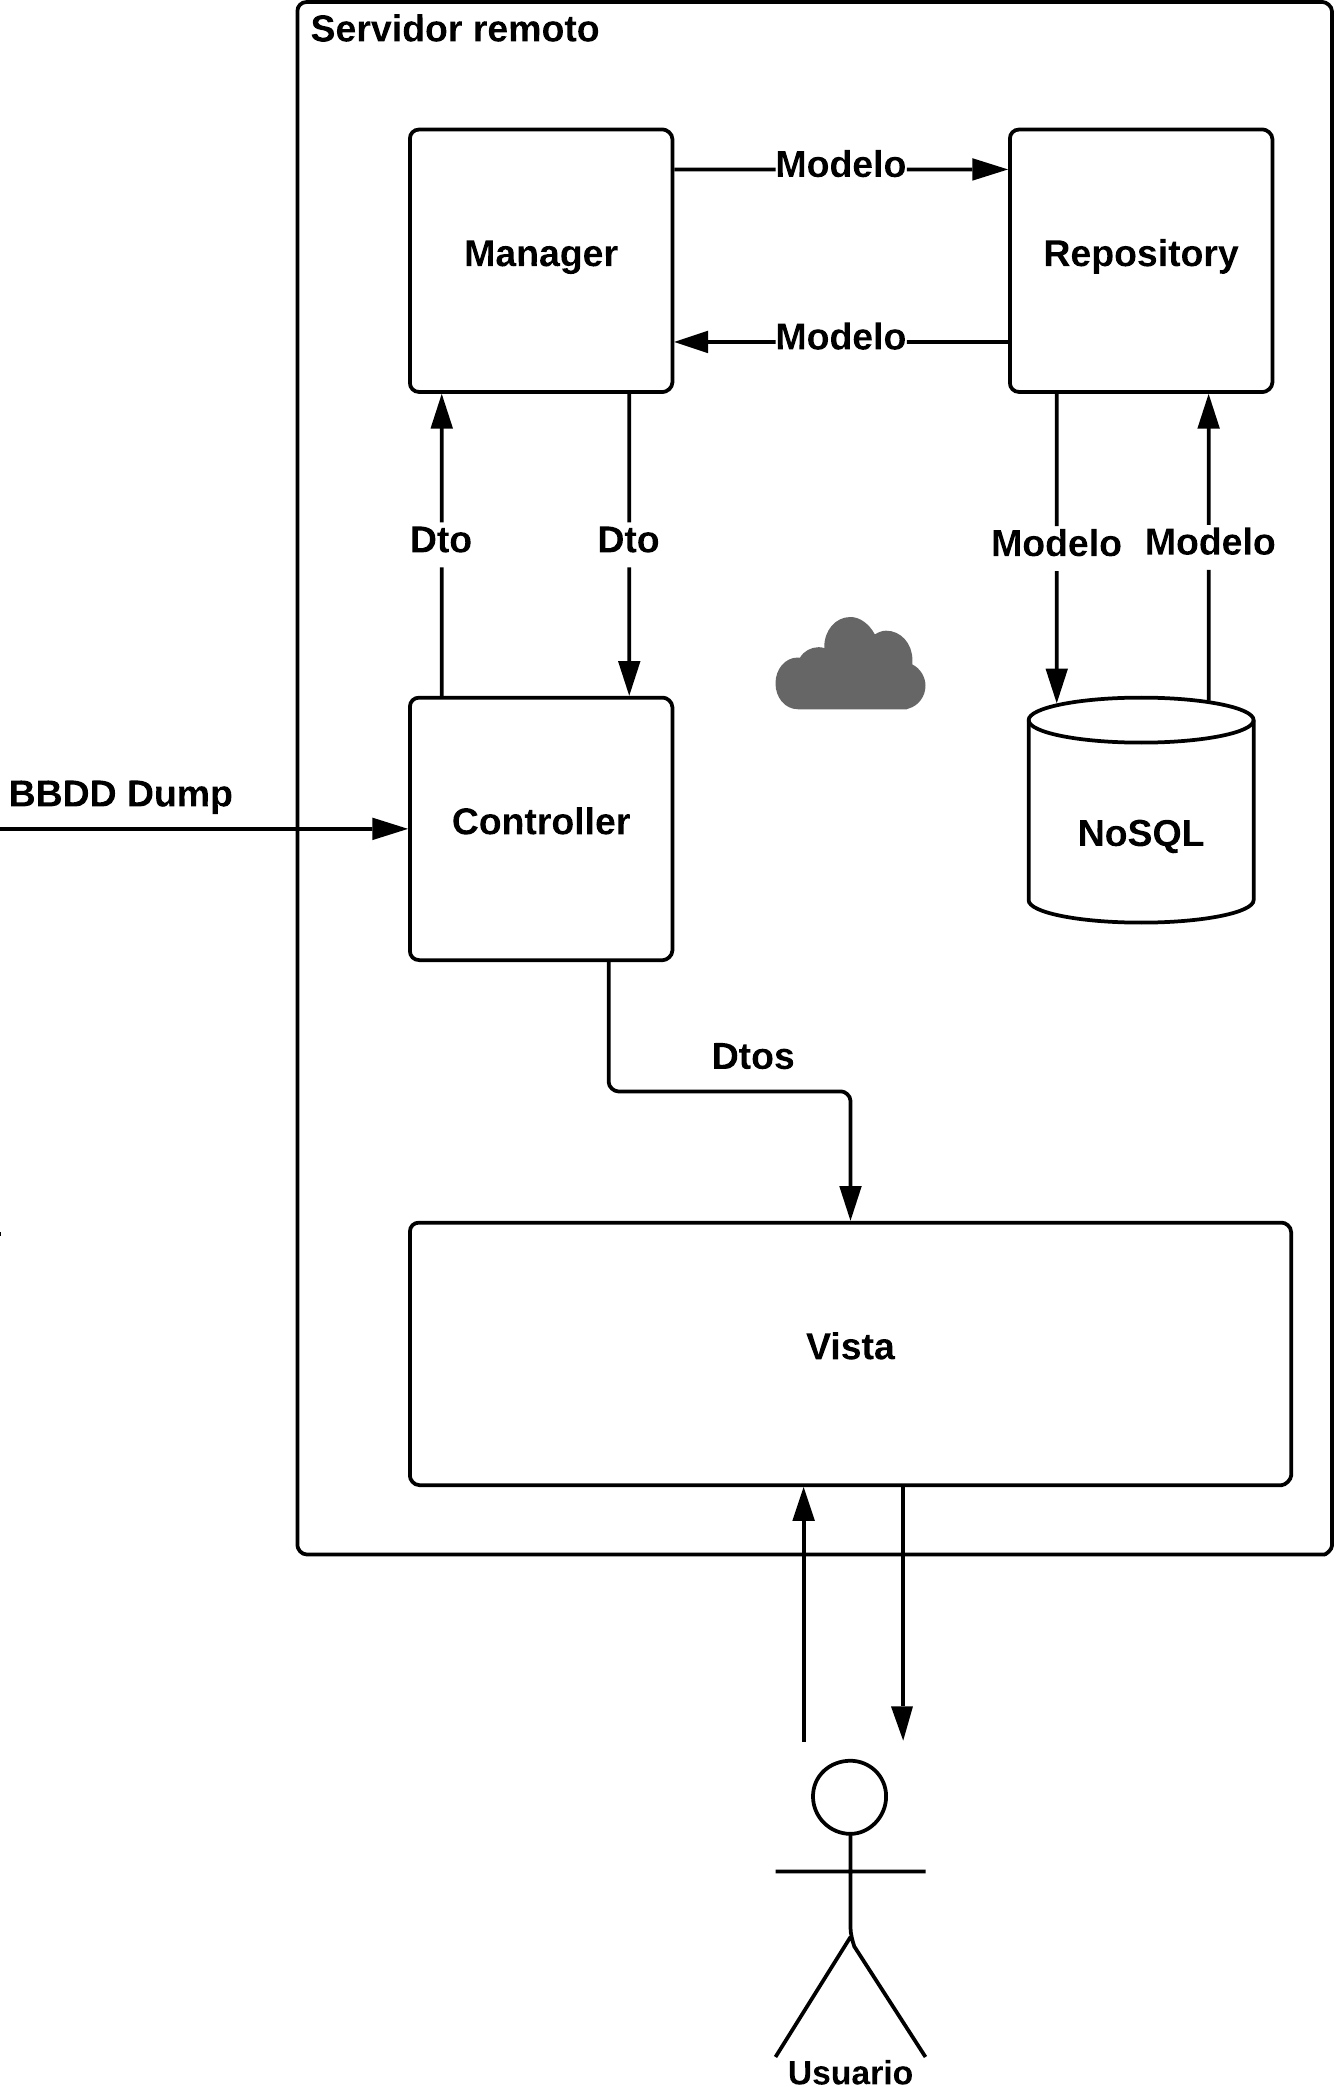
\includegraphics[width=0.5\textwidth]{pictures/architecture/highLevelArch03.png}
  \end{center}
  \caption[Arquitectura de alto nivel. Cloud]{Arquitectura de alto nivel. Detalle del entorno cloud}
\end{figure}
%%% ------
Estamos, por lo tanto, ante una típica arquitectura de servicios web, donde tenemos un controlador, encargado de atender los puntos de entrada de la API, un Manager que realiza las tareas de conversión de objetos y la lógica de negocio, el Repositorio, encargado trabajar contra la base de datos, una base de datos NoSQL y una Vista, 	que nos permite visualizar los datos almacenados. 
\subsubsection{Controller}
Proporciona la interfaz de entrada de la API a través de solicitudes HTTP, así, contaremos con un único método de entrada que aceptará datos en formato JSON, con el contenido en bloques de la base de datos del teléfono, así como los endpoints necesarios para la vista. 
\newline
\newline
Este controller extraerá los datos del json y los convertirá a Dtos, pasándoselos a su vez al manager para que realice la comunicación con las capas inferiores. 
\subsubsection{Manager}
Se encarga de transformar los dtos aportados por el controller en modelos que acepte la base de datos, así como realizar la operación inversa y convertir los datos de la base de datos en Dtos de forma que puedan ser invocados por el controlador y ser devueltos a la vista. 
\newline
\newline
Será por tanto el elemento del entorno cloud donde se depositará toda la lógica de negocio, transformaciones de objetos, mezclados, etc. 
\subsubsection{Repository}
Capa más próxima a la base de datos, nos ofrecerá un sistema de comunicación del resto de la plataforma con la base de datos, siendo este su único punto de entrada, donde manejaremos modelos acordes al esquema de los documentos almacenados en la DB NoSQL. 
\subsubsection{DB NoSQL}
Se trata de nuestra base de datos en la nube, se opta por un sistema NoSQL debido al gran volumen de datos que vamos a manejar. Con el crecimiento de estos datos, surge la necesidad de proporcionar información procesada a partir de grandes volúmenes de datos que tienen unas estructuras horizontales más o menos similares, y este es justo el escenario donde el uso de NoSQL nos brinda la mejor solución. 
\subsubsection{Vista}
Punto de salida de nuestra plataforma cloud, proporcionando así una interfaz de consulta de los datos almacenados, generados por la aplicación. \\
\section{Diagrama de secuencia}
Con el fin de explicar cuál es el flujo que recorren los datos y las operaciones que realiza cada componente así como los mensajes que se intercambian entre ellos, se incluye a continuación un diagrama de secuencia que describe el ciclo de vida de un evento desde el instante en el que se dispara hasta el momento en el que se almacena su información. 
\begin{landscape}
\begin{figure}[htb]
  \begin{center}
     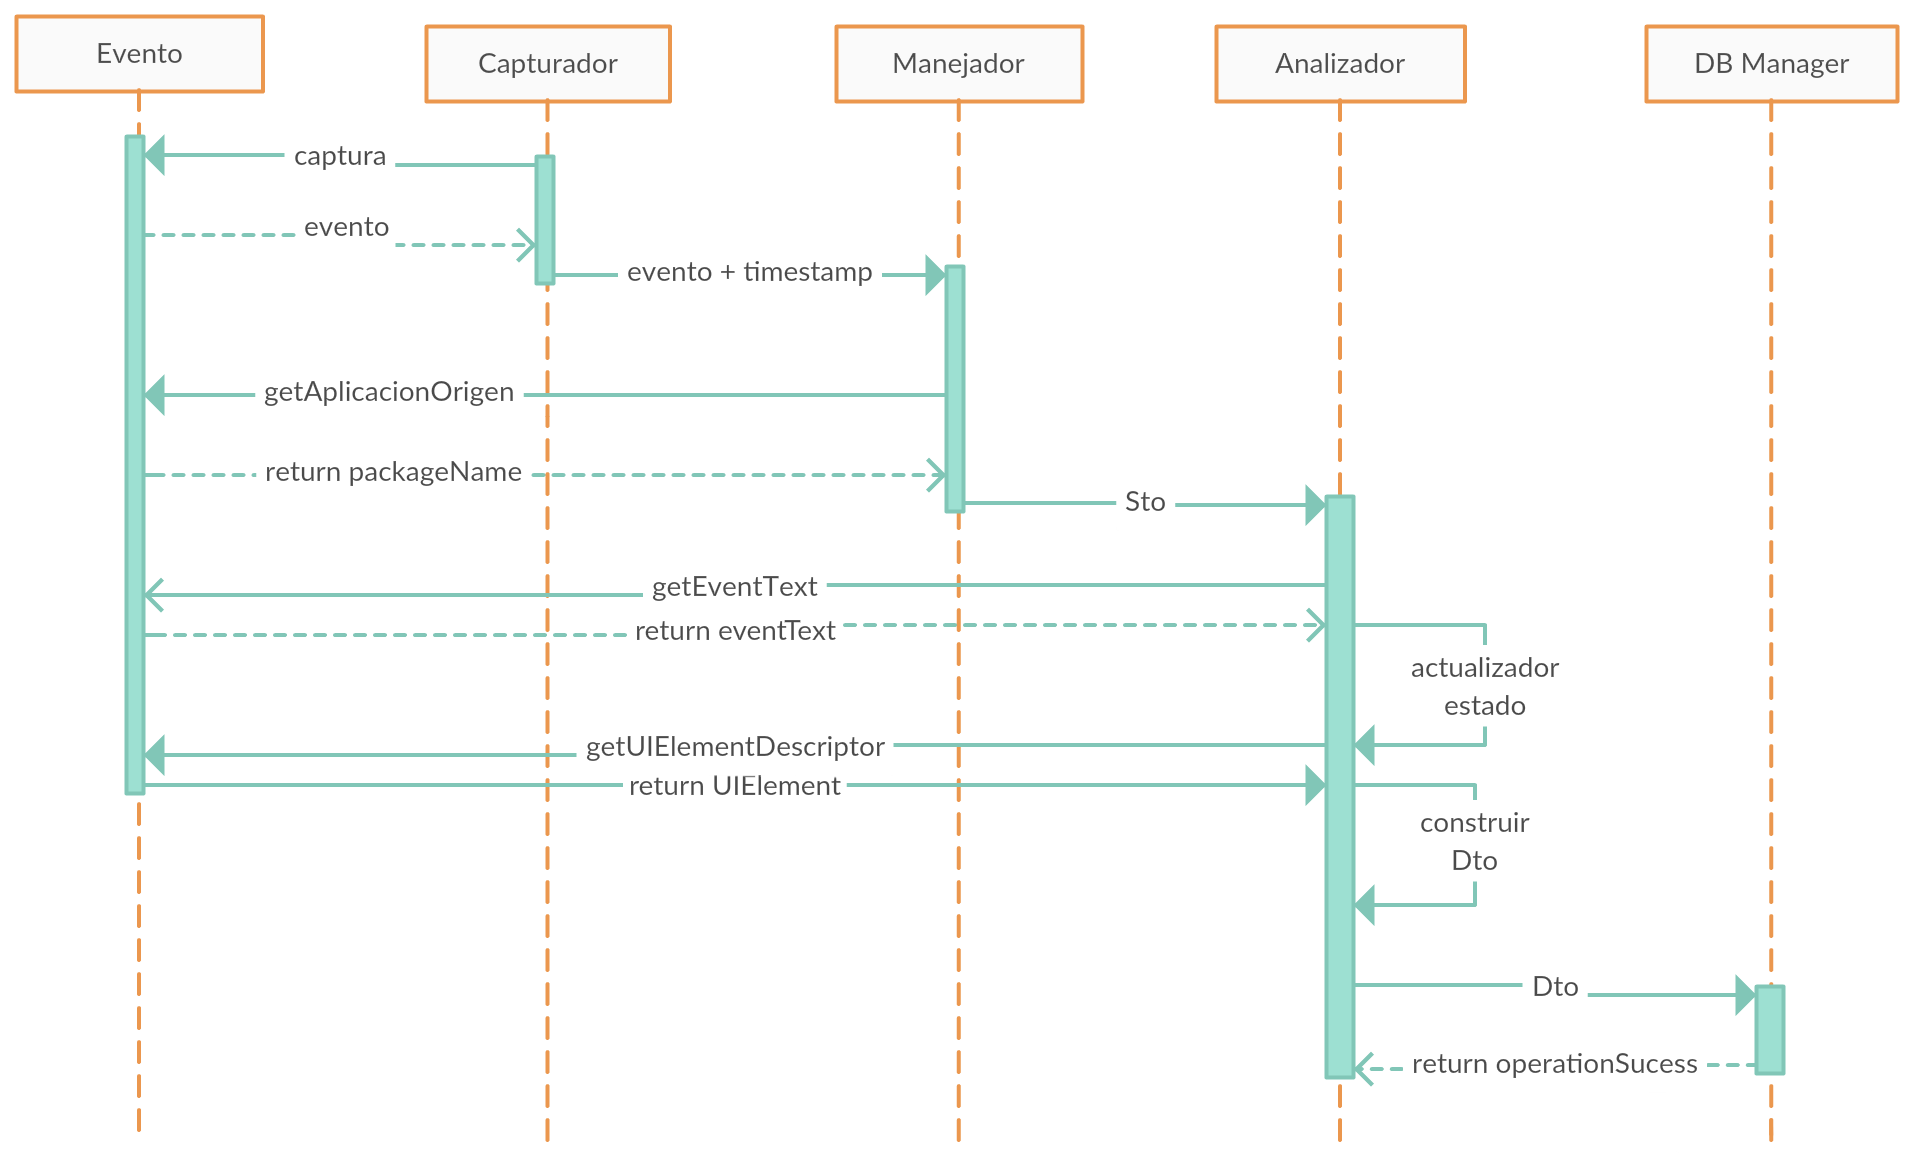
\includegraphics[width=1.5\textwidth]{pictures/secuencediagrams/diagrama_seq_flujo.png}
  \end{center}
  \caption[Diagrama de secuencia]{Diagrama de secuencia habitual del sistema.}
    \label{fig:LandscapeFigure}
\end{figure}
\end{landscape}
\section{Diagramas de actividad}
En esta sección veremos varios diagramas de actividad destinados a clarificar y documentar el flujo lógico que seguirá la aplicación, durante el proceso de análisis y extracción del contenido de cada de las aplicaciones propuestas. 
\subsection{Gmail}
En la siguiente figura se documenta el proceso que lleva al registro de un correo mandado por el usuario a través de la aplicación de GMail. Se ha organizado el diagrama por niveles, desde la capa más externa de la aplicación hasta la capa de persistencia, así se puede observar el camino recorrido así como el procesamiento de la información en cada nivel.
%%% ------ ACTIVIDAD GMAIL 
\begin{landscape}
\begin{figure}[htb]
	\begin{center}
		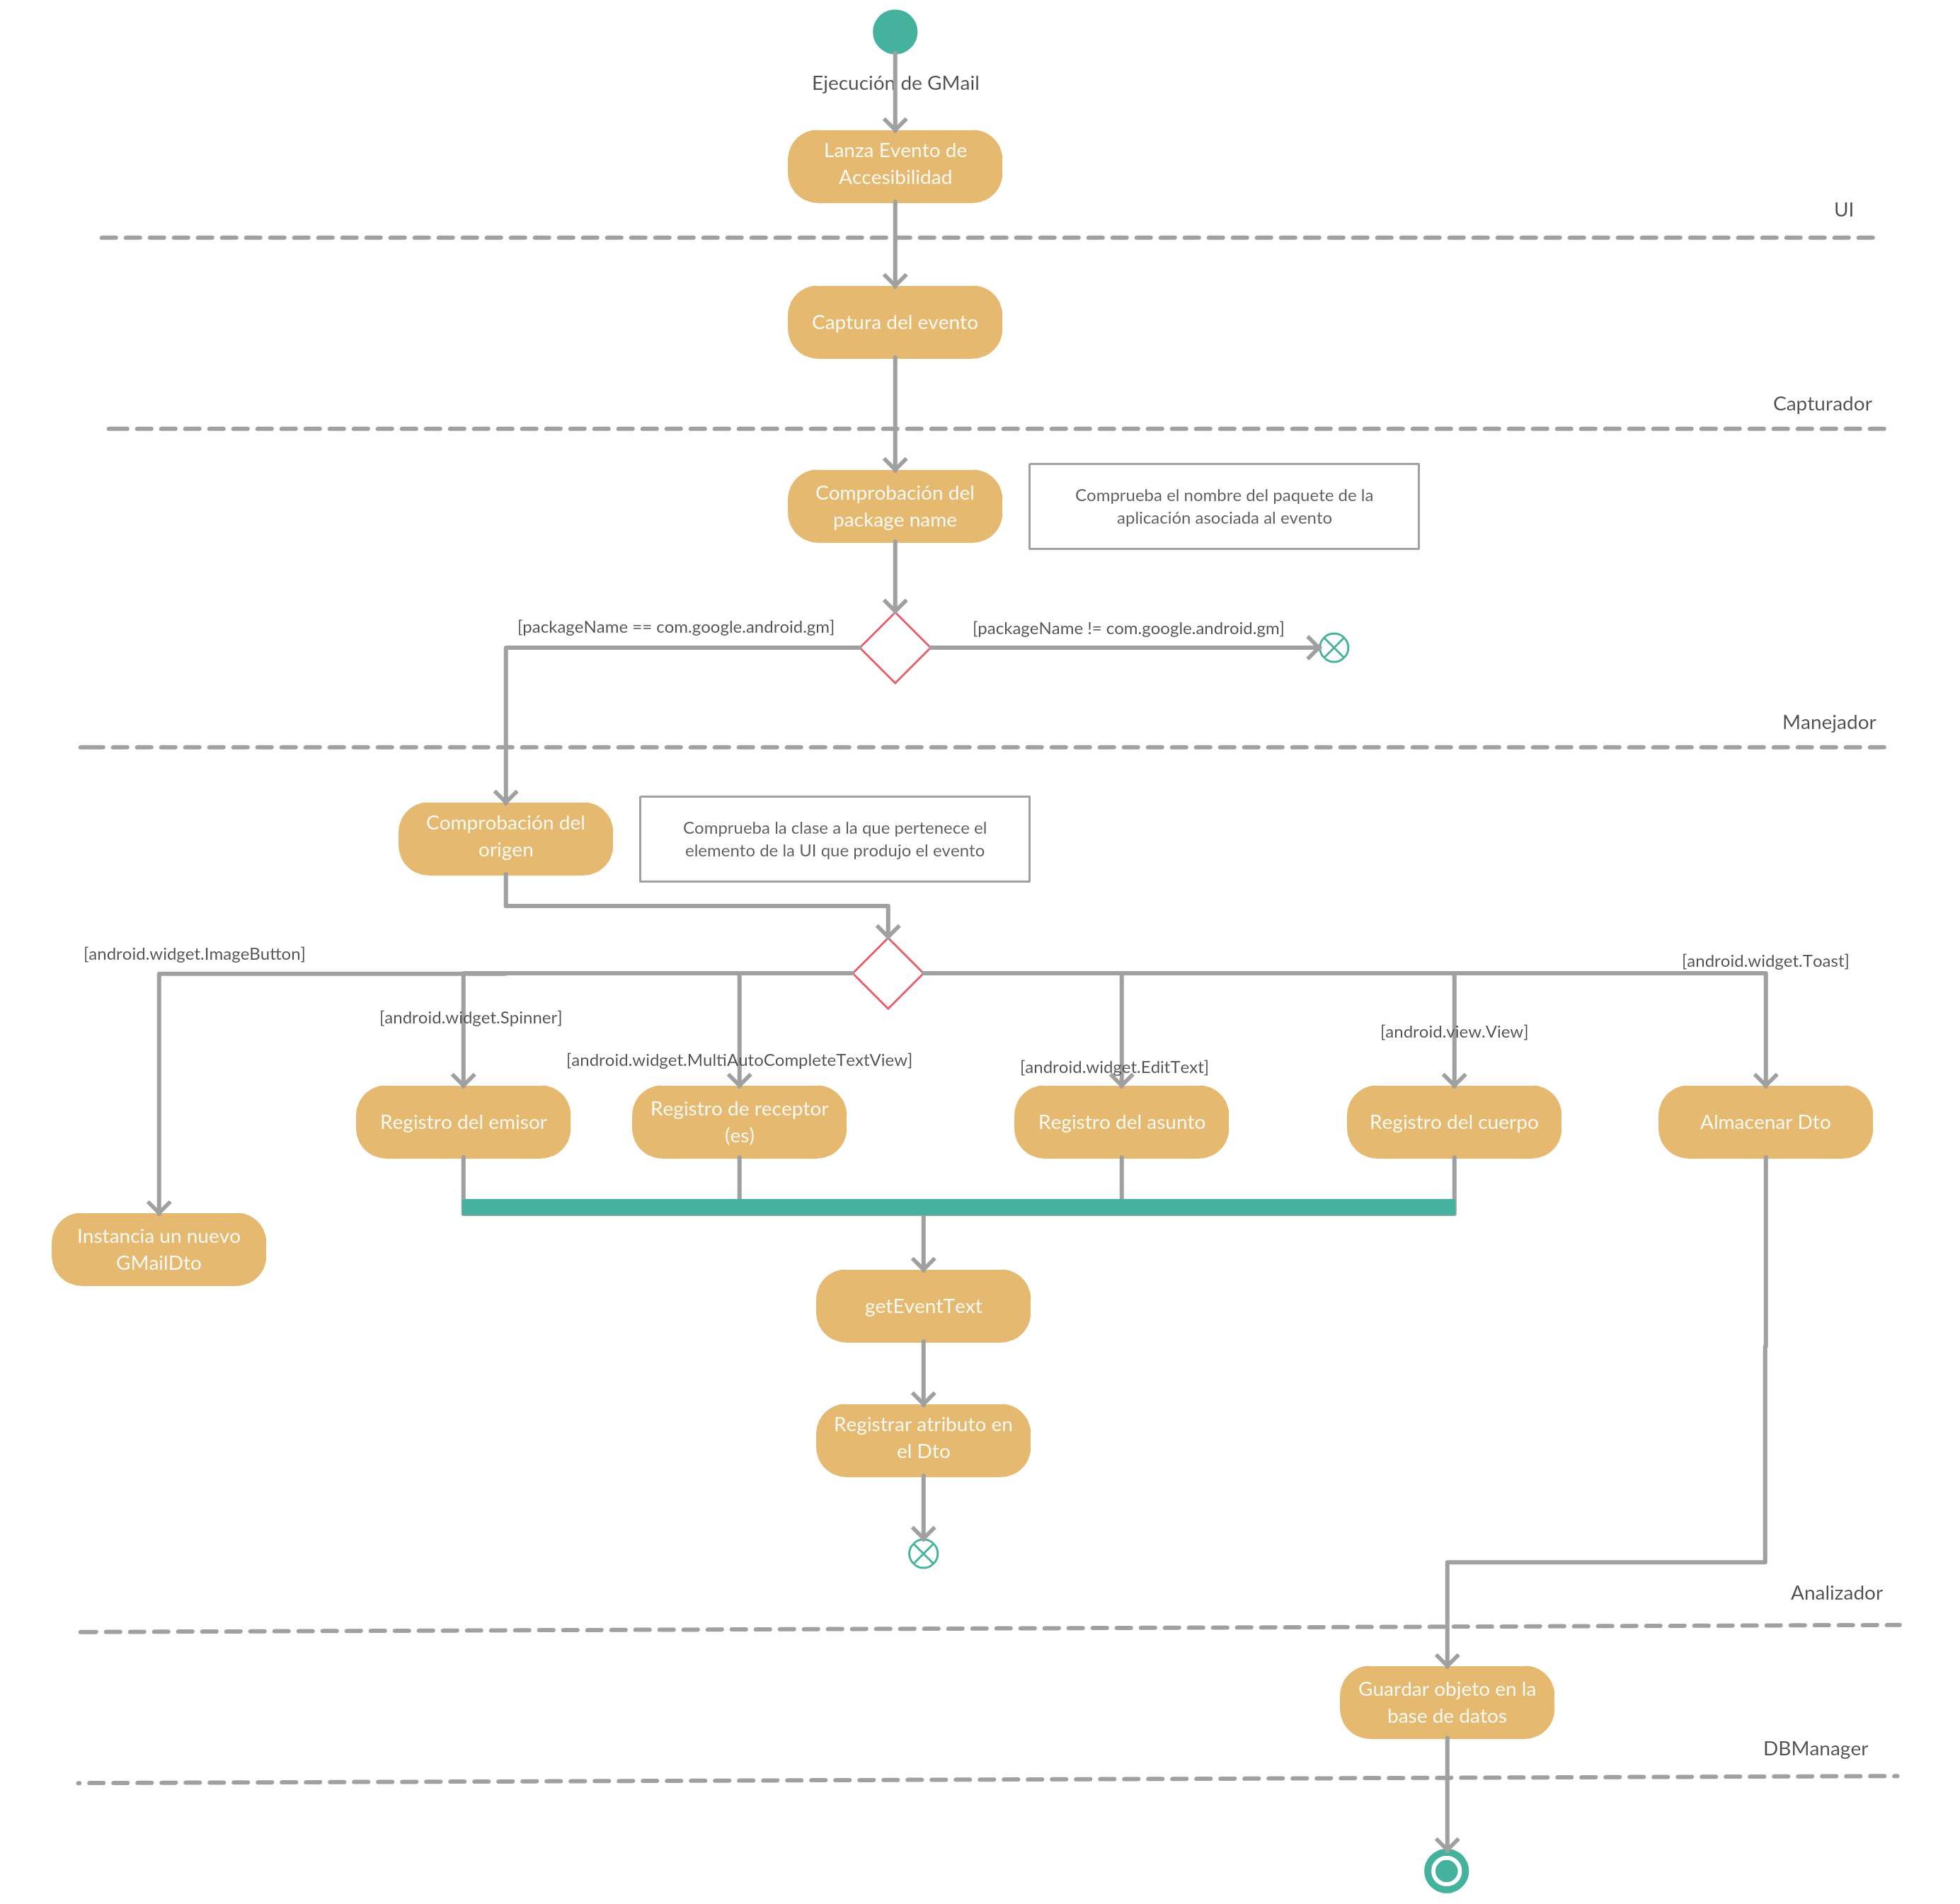
\includegraphics[width=1.1\textwidth]{pictures/activity/gmailActivityDiagram.png} 
	  \caption[Diagrama actividad GMail]{Diagrama de actividad de captura de un correo redactado con GMail.}
	  \label{fig:Diagrama actividad GMail}
  	\end{center}
\end{figure}
\end{landscape}
%%% ------  /ACTIVIDAD GMAIL

 Así, podemos desglosar el proceso en los siguientes puntos, explicando que se hace en cada componente. 
\begin{itemize}
\item \textbf{UI}. En primer lugar, el usuario inicia la actividad al lanzar la aplicación de GMail e interactuar con su interfaz. Esta acción provoca que se lance un evento de accesibilidad por cada elemento gráfico que compone la pantalla. 
% -- item CAPTURADOR
\item \textbf{Capturador}. Actúa como un listener de eventos de accesibilidad, de esta manera está a la escucha de todos los eventos producidos por el sistema, los cuales recoge y junto a la marca horaria del instante de la captura, se lo transfiere al manejador. 
% -- item MANEJADOR
\item \textbf{Manejador}. Comprueba el nombre del paquete que trae consigo el evento, asociado a la aplicación que le dió lugar. En este caso, si el nombre del paquete de la aplicación coincide con el de GMail, \textit{com.google.android.gm}, invoca al analizador de gmail y le delega el evento. 
% -- item ANALIZADOR
\item \textbf{Analizador}. Este es nivel con más carga, puesto que debe comprobar cada evento recibido buscando los componentes de la interfaz conocidos, es decir, aquellos en los que sabemos que se vierte la información que compone el correo. Estos elementos son; 
\begin{itemize}
% -- new subitem
\item \textit{Widget Image Button}. Es el botón de editar que figura en la esquina inferior derecha de la interfaz. 
 	\begin{figure}[htb]
		\begin{center}
     		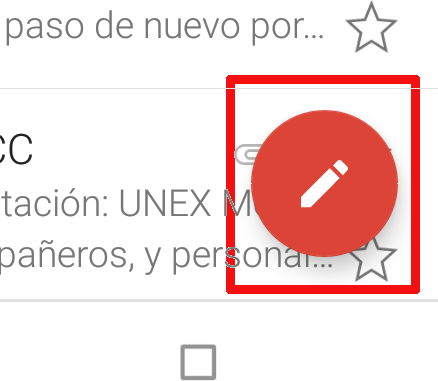
\includegraphics[scale=0.2]{pictures/IRL/GMail/dashboard_gmail_nuevo_correo_cutted.png}
	    	\caption{Android Image Button}{Elemento botón que lanza la creación de un nuevo correo}
    		\label{fig:Android Image Button}
		\end{center}
	\end{figure}
\newline
Al pulsarlo el usuario, el sistema lanza una nueva pantalla en la que redactará el correo. Con lo cual, la pulsación de este elemento de la UI nos inicia el proceso de captura poniendo a nuestro servicio un contenedor, donde compondremos la información del correo. 
\newline
\newline
Cada vez que se pulse este elemento se instanciará un nuevo GmailDto, con el que se trabajará durante el proceso de captura. 

% -- new subitem
\item \textit{Widget Spinner}. Se trata del campo donde aparece el emisor, es decir, el correo del usuario. 
 	\begin{figure}[H]
		\begin{center}
     		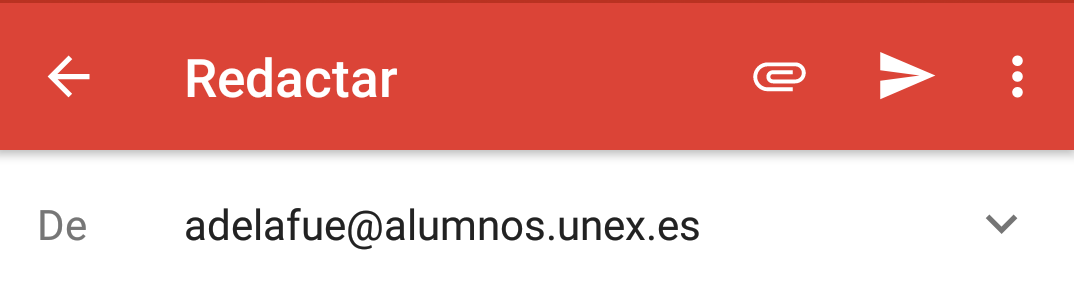
\includegraphics[scale=0.2]{pictures/IRL/GMail/nuevo_correo_gmail_emisor.png}
	    	\caption{Android Widget Spinner}{Elemento gráfico donde aparece el emisor.}
    		\label{fig:Android Widget Spinner}
		\end{center}
	\end{figure}

% -- new subitem
\item \textit{Widget MultiAutoCompleteTextView}. Elemento de la interfaz donde aparecen los receptores, la potencia del componente permite que con las primeras letras del correo del receptor se sugiera la dirección completa.
 	\begin{figure}[H]
		\begin{center}
     		
\includegraphics[scale=0.2]{pictures/IRL/GMail/nuevo_correo_gmail_receptor.png}
	    	\caption{Android Widget MultiAutoCompleteTextView}{Elemento gráfico donde aparece el receptor/es del correo.}
    		\label{fig:Android Widget MultiAutoCompleteTextView}
		\end{center}
	\end{figure}

% -- new subitem
\item \textit{Widget EditText}. Campo de texto donde escribir el asunto del correo. 
 	\begin{figure}[H]
		\begin{center}
     		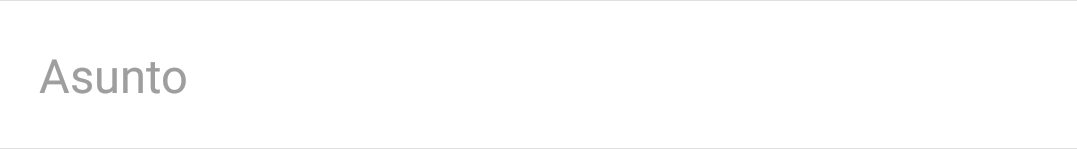
\includegraphics[scale=0.2]{pictures/IRL/GMail/nuevo_correo_gmail_asunto.png}
	    	\caption{Widget Edit Text}{Elemento de la interfaz donde escribir el asunto.}
    		\label{fig:Android Widget EditText}
		\end{center}
	\end{figure}


% -- new subitem 
\item \textit{View}. Vista editable a modo de caja de texto donde se redacta el cuerpo del correo. 
 	\begin{figure}[H]
		\begin{center}
     		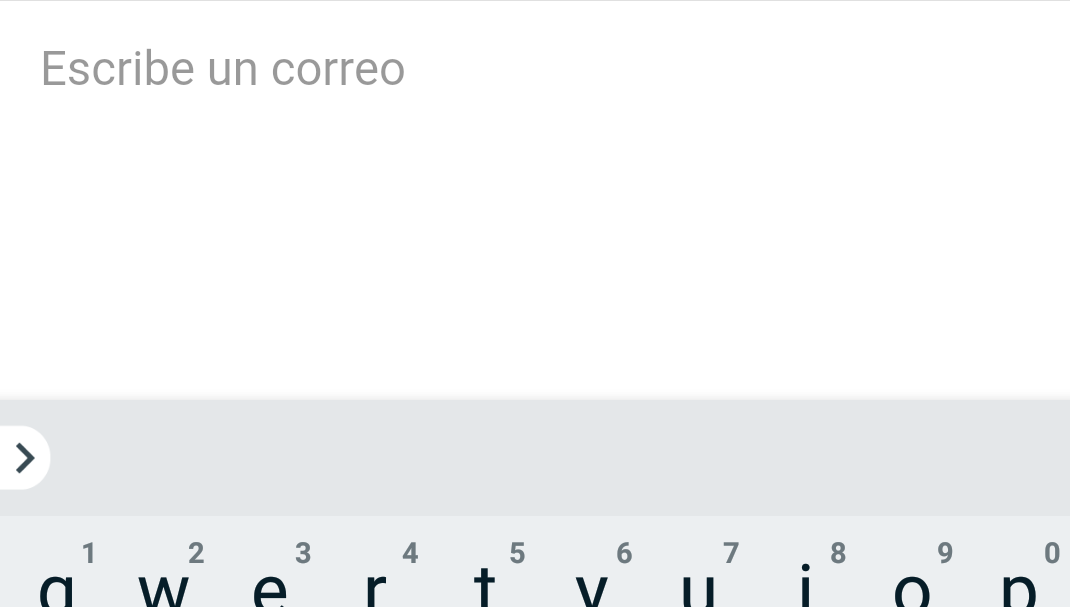
\includegraphics[scale=0.2]{pictures/IRL/GMail/nuevo_correo_gmail_cuerpo.png}
	    	\caption{Android View}{Elemento donde redactar el cuerpo.}
    		\label{fig:Android View}
		\end{center}
	\end{figure}
\end{itemize} % -- elementos de la interfaz
Cada uno de estos elementos descritos sobre la interfaz, generan un evento de accesibilidad que el analizador comprueba a través del nombre de la clase del elemento de la interfaz asociado al evento. Si el nombre coincide con alguno de los elementos aquí listados, se extrae el texto del evento y se infla en el GMailDto el atributo correspondiente (emisor, receptor, asunto y cuerpo). 
Por último, tenemos el elemento \textit{Widget Toast}, típico mensaje que aparece en la mitad inferior de la pantalla que informa de algún suceso. 
\newline
\newline
\begin{figure}[H]
		\begin{center}
     		
\includegraphics[scale=0.2]{pictures/IRL/GMail/correo_enviado.png}
	    	\caption{Android View}{Elemento donde redactar el cuerpo.}
    		\label{fig:Android View}
		\end{center}
	\end{figure}
En este caso el widget toast nos informa cada vez que se envía un correo, momento en el cual cerramos nuestro Dto y se lo pasamos al manejador de la base de datos para que lo persiste en la colección correspondiente. 
\item \textbf{DBManager}. Capa encargada de la persistencia, se encarga mapear los GMailDto a un modelo y almacenarlo en la base de datos local. 
\end{itemize} % -- niveles de app 




 %% #########################
 %% ### ACTIVIDAD WHATSAPP ##
 %% #########################


% -------------- %
% --- DISEÑO --- %
% -------------- % 
\chapter{Diseño}
En este capítulo se detalla el resultado de las sucesivas iteraciones sobre la etapa de diseño. A partir de los requisitos se ha estudiado el problema y planteado una arquitectura que nos permitirá guiar la implementación de los casos de uso. Se pretende obtener una arquitectura limpia y organizada de manera que permita la mantenibilidad del proyecto y una modificación mínima y eficaz. 
\newpage
\section{Arquitectura}
A la hora de plantear nuestra arquitectura el primer paso será conocer la propia arquitectura de Android, por ello, en la siguiente sección estudiaremos como está planteado el sistema sobre el que nos basamos y en base a ese conocimiento tomaremos unas decisiones de diseño que nos ayudarán a componer la arquitectura final. 
\subsection{Decisiones de diseño}
Si nos fijamos en la siguiente figura vemos como Android se asienta en una modificación del Kernel de Linux sobre el que se van abstrayendo capas en las que cada una emplea los servicios que provee la capa inmediatamente inferior. 
%%% ------ 
\begin{figure}[H]
	\begin{center}
		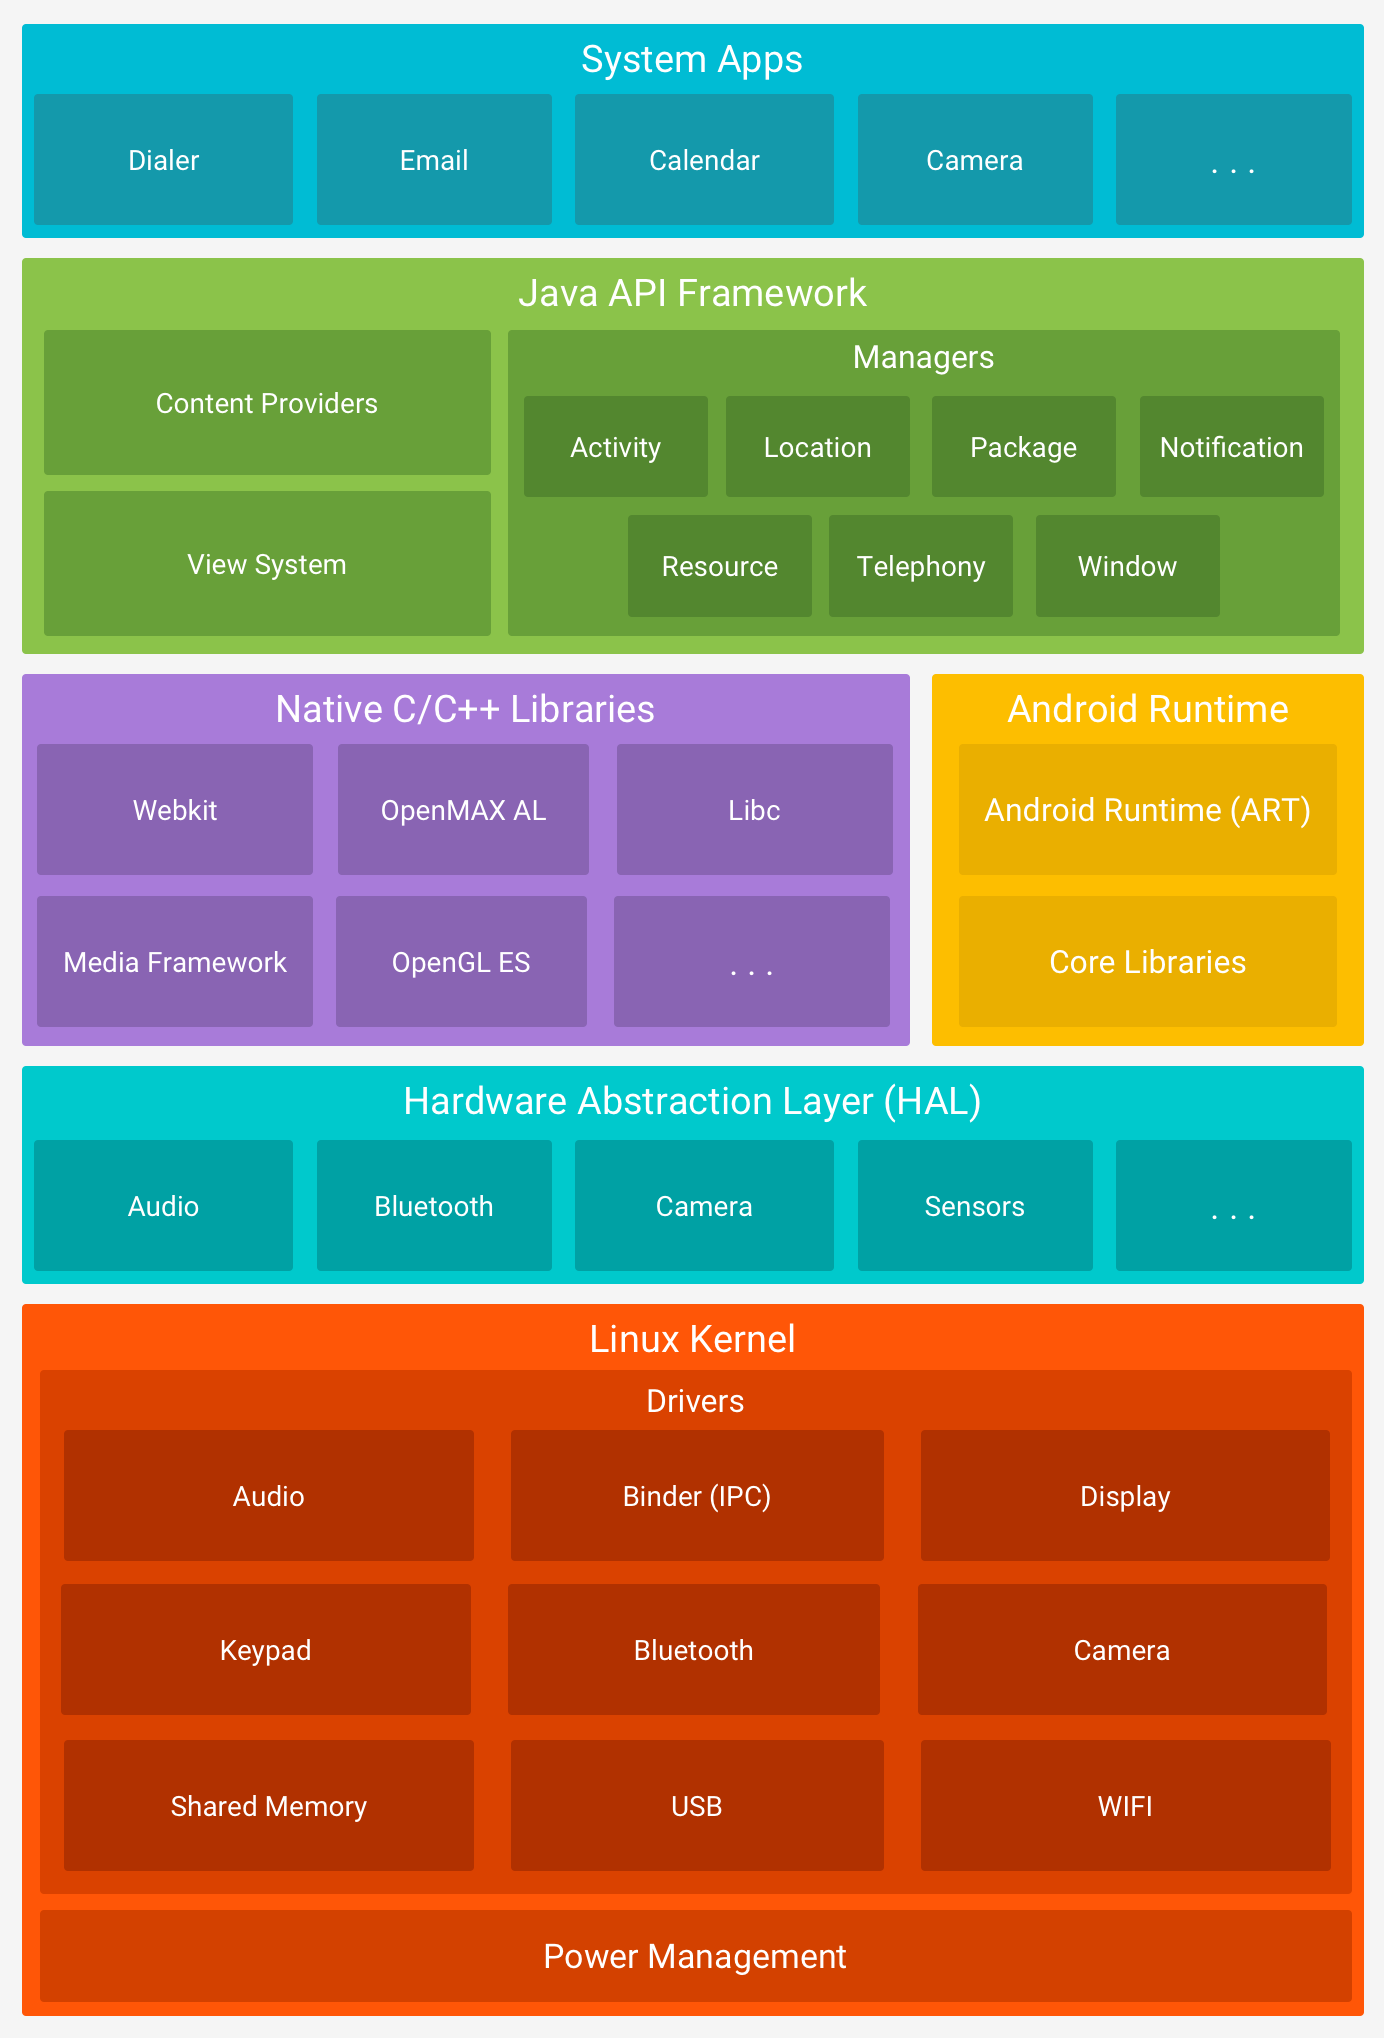
\includegraphics[scale=0.15]{pictures/architecture/android_stack.png} % include ./img/imagen.[pdf|png|jgp] si es pdflatex o ./img/imagen.eps si es latex
	\end{center}
	\caption[Android stack]{Arquitectura por capas de Android.}
\end{figure}
%%% ------
Así, como base de la arquitectura tenemos una modificación del Kernel de Linux sobre la cual se implementa una segunda capa, de abstracción del hardware, que será la encargada de manejar y comunicarse con los periféricos del teléfono. Entendemos por periféricos lo habitual en estos entornos; sensores, antenas, emisores radio...). Sobre estas dos capas, que permiten una interfaz de acceso al dispositivo Hardware, tenemos las librerías de bajo nivel y el entorno de ejecución de android. 
\newline \newline
Si avanzamos un poco más vemos que en las dos últimas capas están relacionadas con una API Java que permite al programador implementar aplicaciones, usando a través de la api, todo la anteriormente expuesto. 
\\
%%% ------ 
\begin{figure}[H]
	\begin{center}
		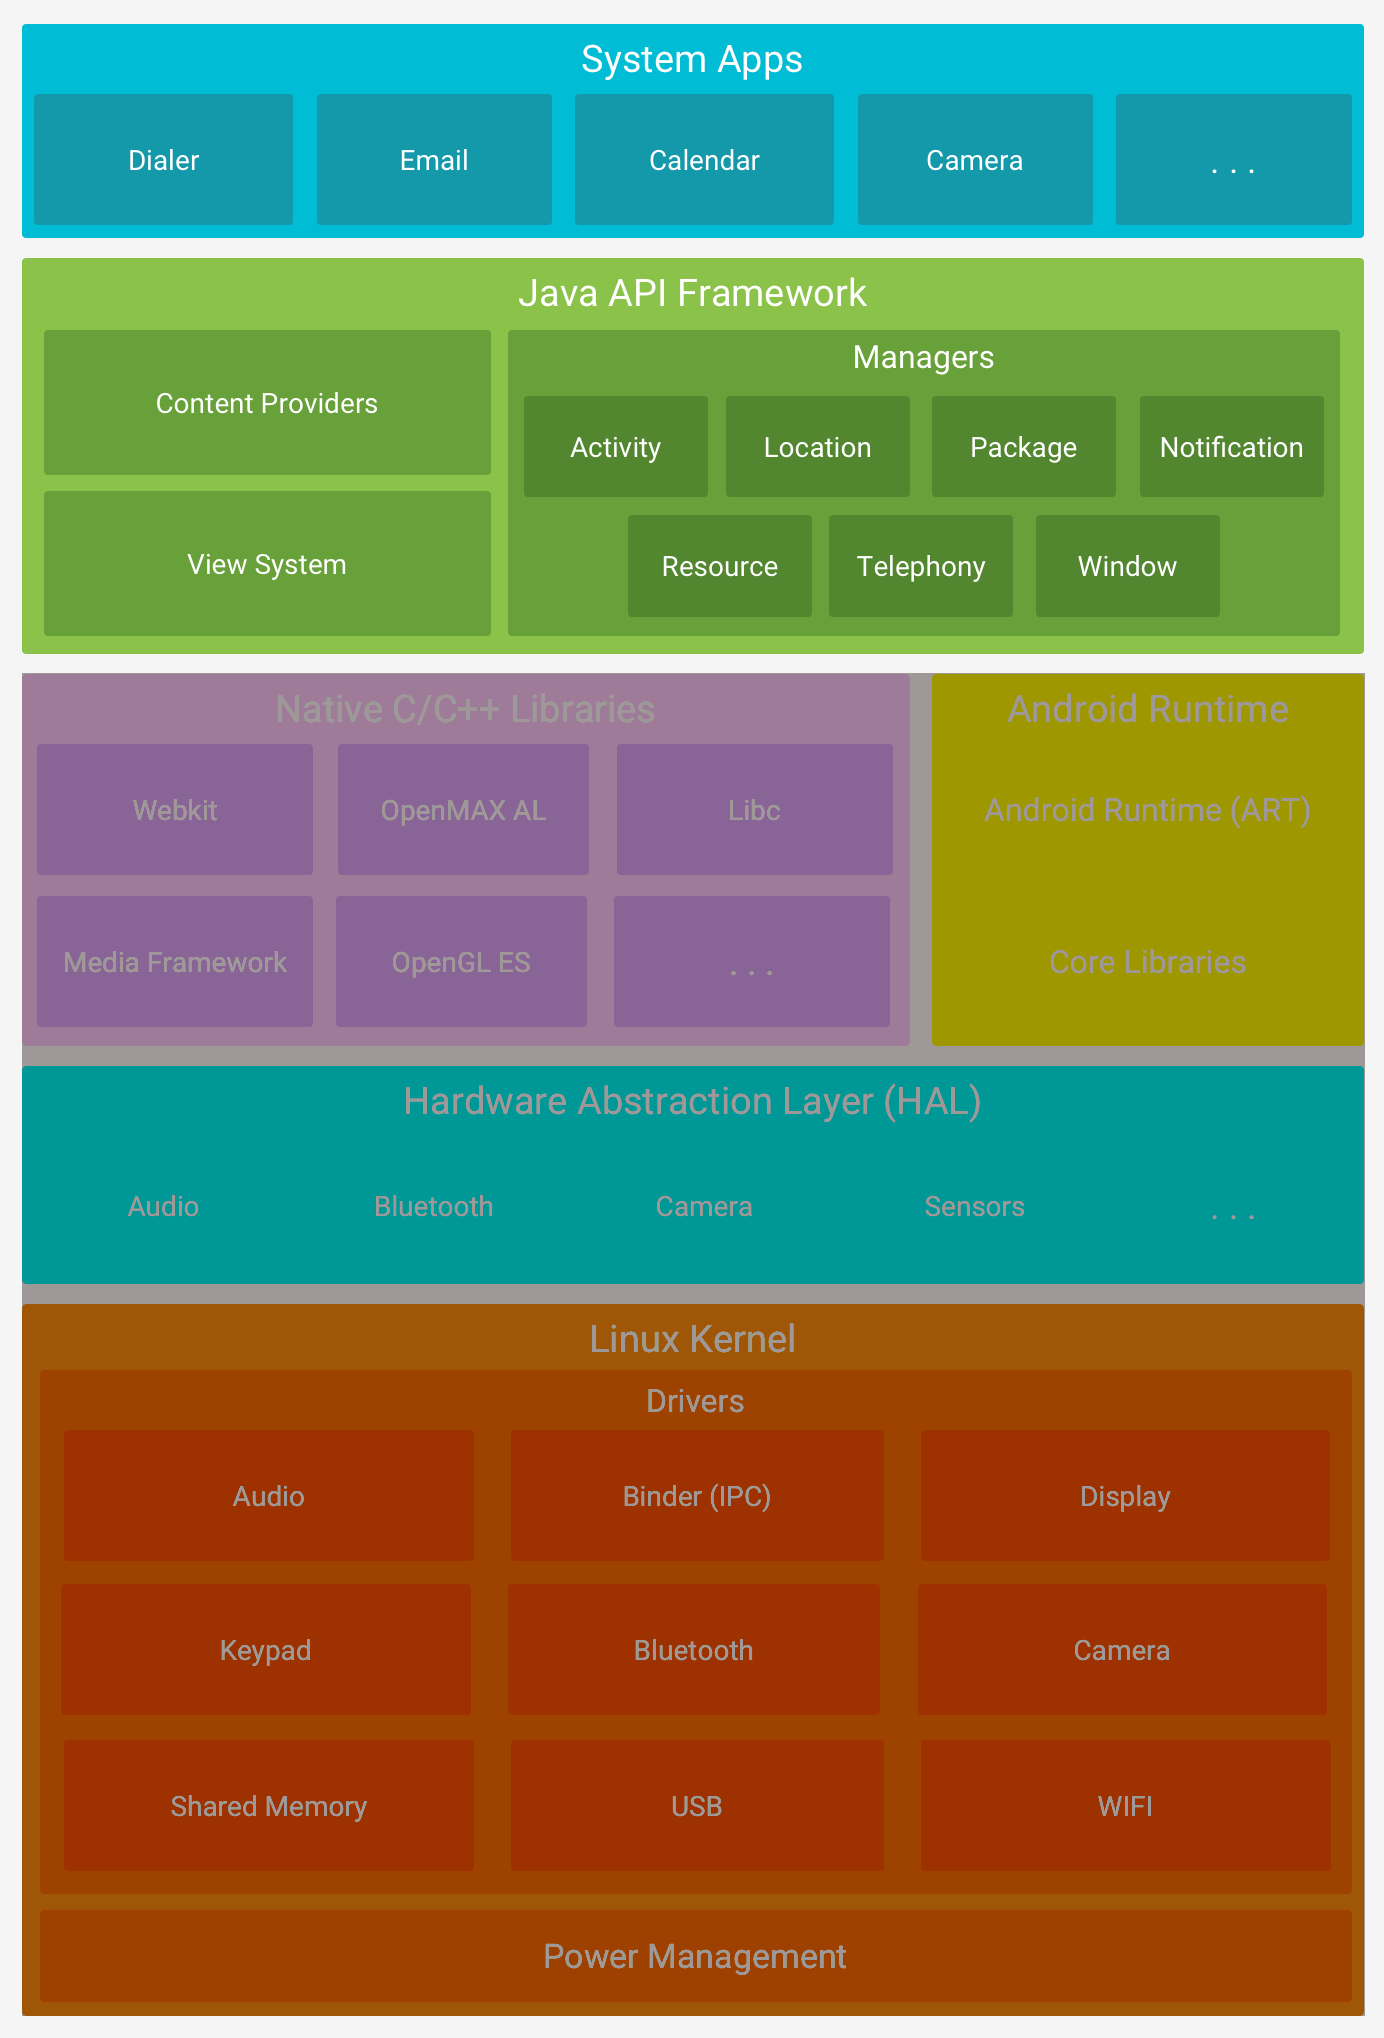
\includegraphics[scale=0.2]{pictures/architecture/android_stack_used.png} 
	\end{center}
	\caption[Detalle del Android Stack]{Márgenes del sistema}
\end{figure}
%%% ------
Estas dos últimas capas serán en las que se situará nuestra arquitectura. Además será conceptualmente parecida puesto que como hemos visto, Android dispone de un sistema organizado por capas, algo bastante lógico y habitual en los sistemas software, y nuestro objetivo por tanto debe ser separar funcionalidades y agruparlas bajo este patrón.
\newline
\newline
Teniendo este concepto claro, nos fijaremos en la publicación de Robert C. Martin, Clean Architecture, en la que se plantea el concepto de Arquitectura Limpia, sin ser más que una serie de condiciones que debe cumplir una arquitectura para que se la considere ”clean". Nos encontramos entonces con una serie de reglas, cuyo cumplimiento ayuda a diferenciar y dividir el software en capas, obteniendo además un software independiente de elementos externos (como la ui, frameworks y bases de datos), testeable y mantenible. 
\newline
\newline
En esta publicación nos encontramos con que una arquitectura debe partir de las entidades (entities). Estas entidades no son mas que las implementaciones sencillas de clases Java. 
\newline
\newline
Estas clases permitirán instanciar objetos que reprensentarán a los actores principales de la lógica de negocio. Por tanto POJOS (Plain Old Java Object) y Dtos (Data Transfer Objects) se verán incluidos en esta capa. 
%%% ------ 
\begin{figure}[H]
	\begin{center}
		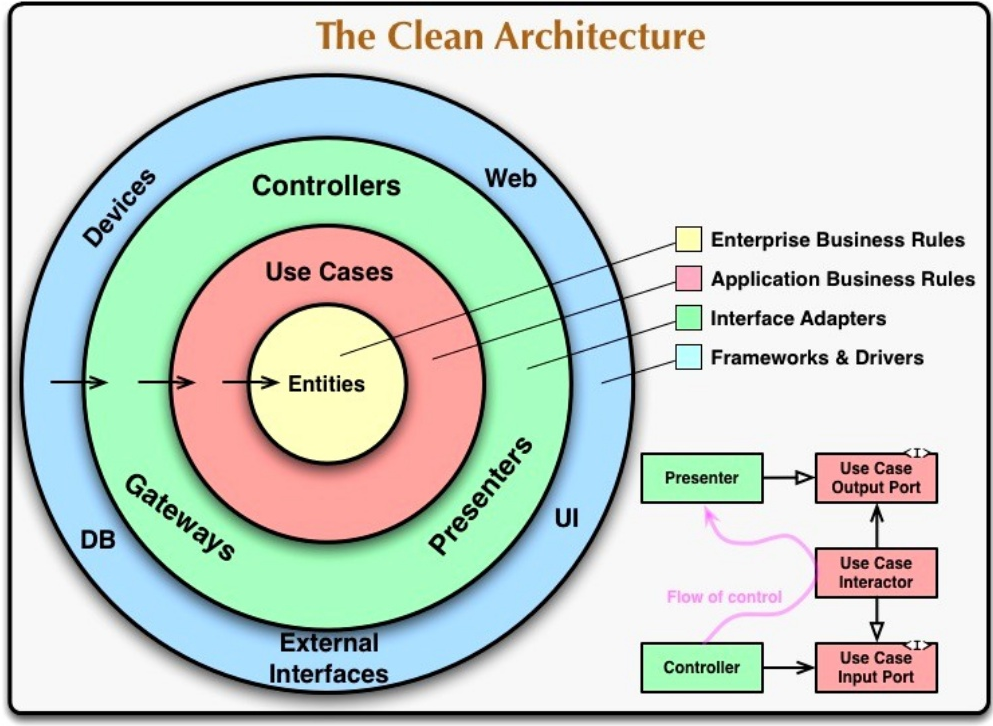
\includegraphics[scale=0.3]{pictures/architecture/android_architecture.png} 
	\end{center}
	\caption[Clean Architecture]{Arquitectura clean}
\end{figure}
%%% ------ 
Los casos de uso (use cases) están muy relacionados con las entidades, puesto que implementarán la lógica de negocio del sistema, orquestando y orientando el flujo de datos del sistema. 
\newline
\newline
La capa de los Interface Adapters realiza la conversión de los datos de manera que se puedan comunicar los niveles superiores con los casos de uso y entidades (en MVC corresponde a los Controladores, MVVP al presenter... etc). 
\newline
\newline
En la última capa y más externa, Frameworks and Drivers, residen las plataformas y herramientas externas, donde se incluye la interfaz de usuario, web... 
\subsection{Arquitectura a bajo nivel}
Una vez tenemos claro como está estructurado Android y los servicios que ofrece al desarrollador, debemos plantearnos cómo diseñar una aplicación que sea capaz de implementar estos servicios de accesibilidad para capturar, procesar y extraer la  información de los eventos que se generan, deberemos abstraernos del problema y ser capaces de, a partir de una vista general del sistema inferir las capas que finalmente nos guiarán la implementación. 
\newline
\newline
Así pues, en primer lugar situar nuestro sistema dentro del stack tecnológico de Android citado al principio de esta sección. 
\newline
%%% ------ 
\begin{figure}[H]
	\begin{center}
		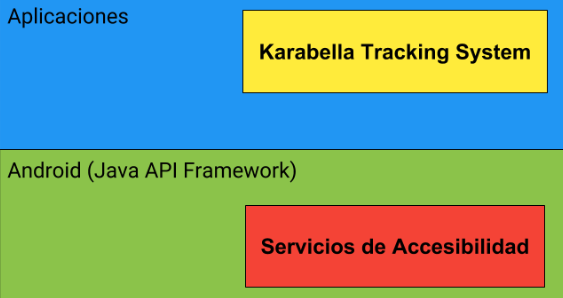
\includegraphics[scale=0.6]{pictures/architecture/arquitecturaGeneral01.png} 
	\end{center}
	\caption[Arquitectura dentro del android stack]{Arquitectura del sistema dentro del stack de Android.}
\end{figure}
Es natural esta clasificación puesto que el proyecto se basa en la implementación de los Servicios de Accesibilidad que Android dispone en de su API, gracias a mecanismos como la herencia y la implementación de interfaces. 
\newline \newline
Estos servicios de accesibilidad son la solución de Google para asistir y dar soportes a usuarios con diversidad funcional. Su naturaleza y comportamiento es lo que nos permite aprovechar estos servicios para obtener información de lo que hace el usuario. 
\newline \newline
Se comporta además como cualquier otro servicio de Android, (es decir, procesos ideados para correr en segundo plano con un ciclo de vida prolongado en el tiempo). El Servicio de Accesibilidad se comporta como listener de Eventos de Accesibilidad, que lanzados por el sistema, son recogidos por la clase que implemente este servicio, donde son capturados y tratados como mejor convenga. Estos eventos serán, entonces, la unidad de información más básica que manejará nuestro sistema, pero a la vez la más compleja, dado que llevan dentro toda la información sobre la cual se construyen el resto de capas.
\newline \newline
Los eventos llevan consigo información sobre la interfaz de usuario, por ejemplo los eventos se lanzan cuando entra en foco un elemento (con la descripción del elemento, botones, entradas de texto, nombres de ventanas...). Nuestra solución pasa por extraer la información de esos eventos y procesarla. 
\newline \newline
Dado que estos eventos pueden ser capturados por Eventos de Accesibilidad, nuestro sistema contará con un servicio que lo implemente y que realiza esta captura, este será un elemento fundamental en la arquitectura puesto que será la base sobre la que se asentarán el resto de elementos. 
\\
Así, en un primer vistazo, podemos ver la arquitectura usando un grano gordo del siguiente modo. 
%%% ------ 
\begin{landscape}
\begin{figure}[htb]
	\begin{center}
		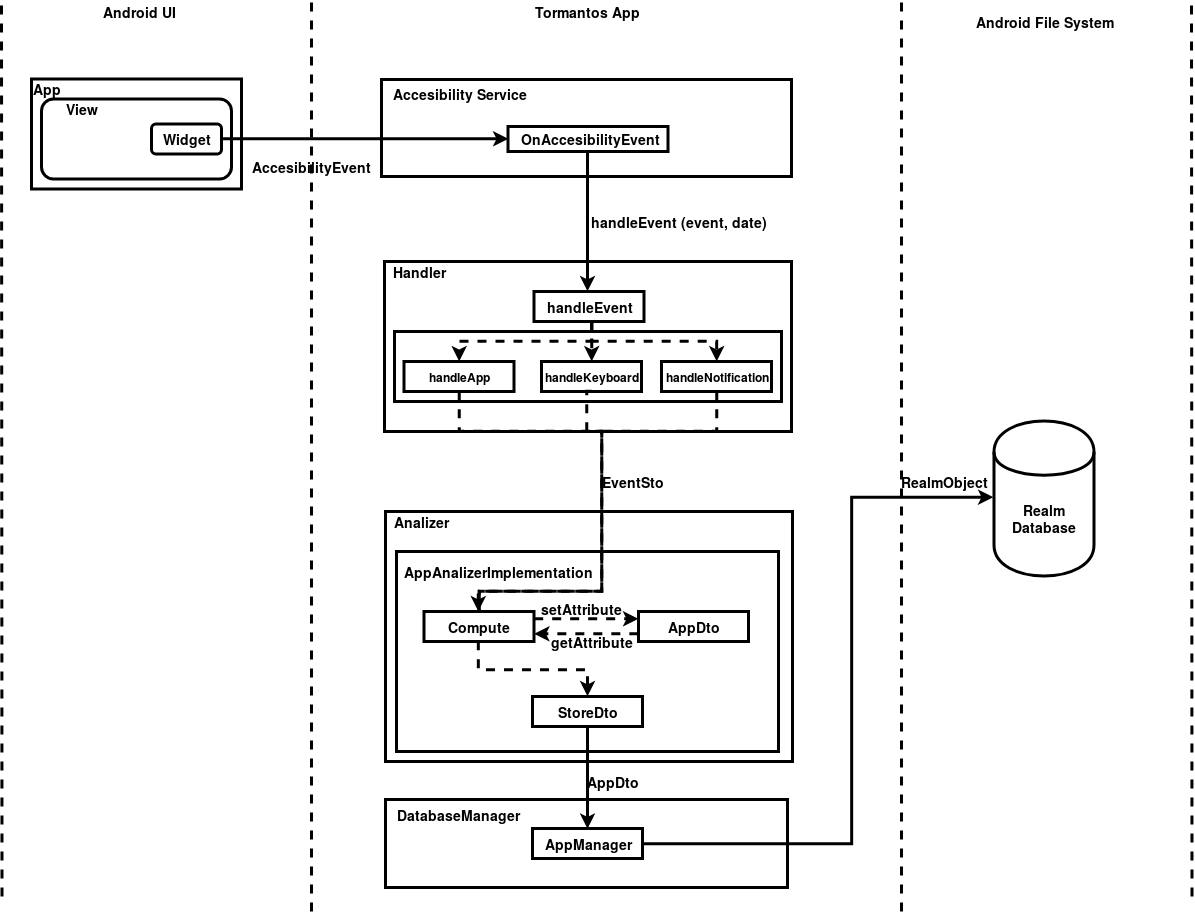
\includegraphics[scale=0.45]{pictures/architecture/lowLevel/TFG_ArquitecturaBajoNivel01.png} 
	\end{center}
	\caption[Arquitectura general del sistema]{Arquitectura general del sistema}
\end{figure}
\end{landscape}

%%% ------ 
Donde la interfaz de usuario (UI) genera eventos de accesibilidad. Estos eventos, como ya se ha comentado, están asociados a cada acción que el usuario realiza con el teléfono sobre la interfaz. Será la implementación del evento de accesibilidad (Accesibility Service) el que nos permita capturarlos. 
\newline
\newline
Este servicio se encargará de capturar los eventos y mandarlos hacia el Manejador de Eventos (Event Handler), este manejador será el encargado de clasificar y procesar los eventos en función de la información que traigan consigo. 
\newline
\newline
Una vez que estos eventos pasen por el manejador, obtendremos como resultado una entidad lista para ser guardada en la base de datos. 
\newline
\newline
Profundicemos un poco más en como sería este manejador y como son los componentes que lo forman. 
\newline
\newline
Como estamos viendo, el servicio de accesibilidad (lo llamaremos simplemente servicio) recibe eventos de la interfaz y los envía al manejador, pero dado que los eventos se generan en gran cantidad y en momentos puntuales tendremos que manejar un caudal de información importante, la comunicación entre el servicio y el manejador se realizará a través de un bus que permitirá al servicio desatender los datos lo antes posible y desentenderse así de lo que ocurre con esos datos y como son tratados.
\newline
\newline
Este bus lo estará escuchando el manejador, que capturará los elementos para realizar un primer chequeo, y es que en función del nombre de la aplicación (más concretamente su package name), invocará a un \textit{Scraper} encargado de extraer la información relevante del evento que estamos manejando. 
\newline
\newline
En nuestro sistema tendremos una interfaz Analizer, con tantas implementaciones como aplicaciones estemos monitorizando. Procesarán el evento de accesibilidad y lo encapsularán en una unidad de datos que será pasada a la capa de persistencia, formada por los Managers. Encargados de persistir en una base de datos local los datos generados por el sistema. 
\newline
\newline
Al final nuestra arquitectura a bajo nivel resulta en el siguiente diagrama. 
%%% ------ 
\begin{figure}[H]
\begin{center}
		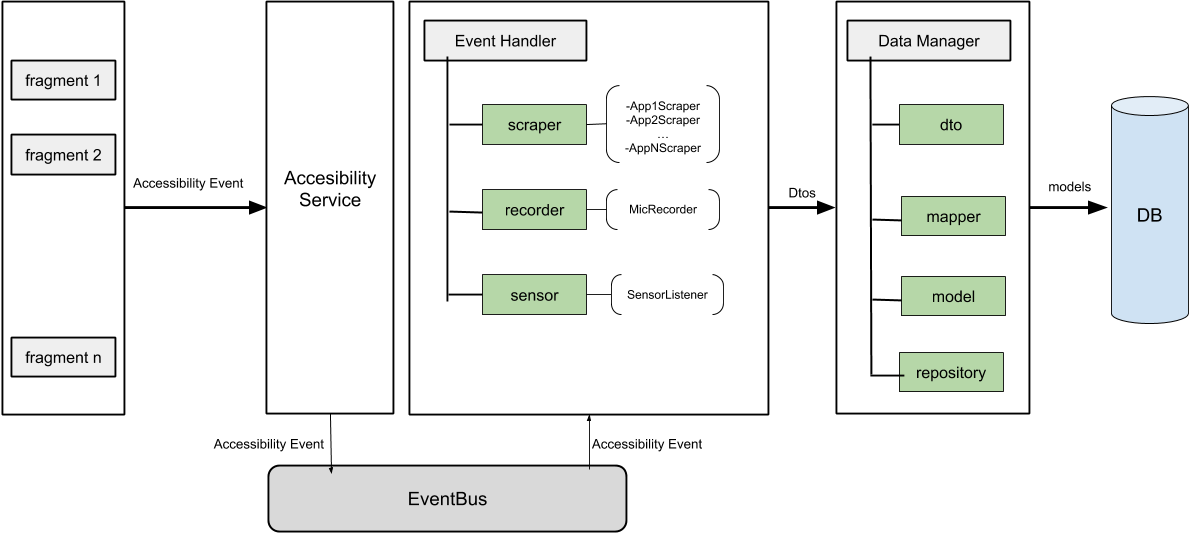
\includegraphics[width=1.3\textwidth]{pictures/architecture/arquitecturaGeneral03.png} 
%	\end{large}
	\caption[Arquitectura detallada]{Arquitectura detallada}
	\end{center}
\end{figure}
%%% ------  
En primer lugar nos encontramos la ui que alimenta al servicio de accesibilidad con eventos. Este servicio se encarga de meterlos en un bus de forma que el manejador pueda recogerlos y computarlos. 
\newline \newline
Este tratamiento que realiza el manejador no es otro que, en función de la app que lo lanzó llamar a las clases implicadas en su tratamiento.
\newline \newline
Expliquemos más despacio en que consite esto. El manejador, como se ha dicho en alguna ocasión, analiza el package name del evento, este package name nos permite identificar el elemento del sistema android que lanzó el evento, ya sean relacionados con la aplicación en foco en ese momento como los relacionados con el uso de sensores del teléfono. 
\newline \newline
Los eventos de las aplicaciones serán tratados por el analizador que le corresponda. Estos extraerán la información pertinente y la encapsularán en dtos. 
\newline \newline
Con los sensores la historia es diferente, puesto que la escucha de los mismos está ligada a la implementación de sendos listeners que recogen la información que van generando. En un apartado diferente entra la escucha del micrófono, puesto que para respetar la privacidad del usuario sólo se lanzará la captura de audio cuando un evento relacionado con la misma sea lanzado. Nos referimos a casos concretos del uso del móvil como comandos de voz, notas de audio, etc. 
\newline \newline
En la parte del Data Manager nos encontramos a las entidades y a los responsables de mover esas entidades a lo largo de la arquitectura. 
\newline \newline
Así nos encontramos con el paquete repository, encargado de la persistencia en base de datos de las entidades. Entidades como dtos (para la comunicación de información desde el manejador al data manager) y mappers, que realizarán la conversión de dtos a modelos, entidad aceptada por el repository para la persistencia en la base de datos. 
\newline \newline
De esta manera nos encontramos con 4 capas separadas por funcionalidad y con independencia lógica entre ellas, puesto que cada una está consagrada a una tarea particular (recibir eventos, computarlos, persistirlos). 
\newline \newline
La lógica de negocio del sistema se encuentra, sin duda, en la capa correspondiente al manejador, donde deberemos de echar un esfuerzo de implementación considerable para manejar todo el flujo de información. 
%%% ------


\chapter{Implementación y desarrollo}
\section{Bibliotecas de terceros}
\subsection{Realm}
Realm es una base de datos cuya implementación para Android nos ofrece una alternativa a SQLite, destactando por su rapidez y facilidad de uso. 

Se trata de una base de datos orientada a objetos, facilitando así el mapeo objeto relacional a través del código, incluyendo de esta manera las facilidades de un ORM de forma nativa. 
\newline \newline
Para añadirla su dependencia basta con añadir en el build gradle (Project): 
\begin{verbatim}
		classpath "io.realm:realm-gradle-plugin:5.1.0"
\end{verbatim}
En este caso se está usando exactamente la versión 5.1.0. Deberemos añadir en el build gradle (App): 
\begin{verbatim}
		apply plugin: 'realm-android'

\end{verbatim}




%~\ref{fig:Calculo IDLE-PC} este valor es calculado automáticamente por el programa, algo que no pasa en versiones anteriores de este, donde se calculan varios valores que se muestran al usuario para que este seleccione uno de ellos.
%\begin{figure}[h]
%\centering
%\caption[Calculo IDLE-PC]{Calculo IDLE-PC}
%\label{fig:Calculo IDLE-PC}
%\end{figure}


\chapter{Conclusiones y trabajos futuros}


%%%%%%%%%%%%%%%%%%%%%%%%%%%%%%%%%%
%%%%%%%%%%% ANEXOS %%%%%%%%%%%%%%%
%%%%%%%%%%%%%%%%%%%%%%%%%%%%%%%%%%
%%\appendix
%%%\clearpage
%%\appendixpage
%%%\addappheadtotoc

%%%%%\chapter{Ejemplo de anexo}
%%%%%%Si no se desea incluir anexos, sólo hay que borrar este capítulo.
%%%%%\par



\pagebreak
%%%%%%%%%%%%%%%%%%%%%%%%%%%%%%%%%%
%%%%%%%%%% AL FINAL %%%%%%%%%%%%%%
%%%%%%%%%%%%%%%%%%%%%%%%%%%%%%%%%%
\thispagestyle{empty}
\pagestyle{empty}
%%%% https://en.wikibooks.org/wiki/LaTeX/Bibliography_Management
\bibliography{bib}

\bibliographystyle{plain}
\end{document}
%%%%%\section{Secciones}
%%%%%Las secciones se crean con \textit{section}. Las subsecciones y %%%%subsubsecciones con \textit{subsection} y \textit{subsubsection}, %%%%respectivamente. Si se desea que alguna subsección en concreto no salga %%%%en el índice se pueden usar los mismos comandos añadiéndoles un %%asterisco al final (\textit{subsection*} y \textit{subsubsection*}).
%%\par

%%%%%\subsection{una subsección}

%%%%%%\subsection{otra subsección}
%%%%%%Excepteur sint obcaecat cupiditat non proident, sunt in culpa qui %%%%%%officia deserunt mollit anim id est laborum.
%%%%%%\subsubsection{subsubsecciones}
%%%%%%¡Por defecto las subsubsecciones no aparecen en el índice! Este %%%%%%comportamiento se puede cambiar.

%%%%%%\section{Citas y referencias}
%%%%%Para citar un texto hay que incluirlo en el fichero %%%%\textit{LocalBibliography.bib} de esta plantilla. Una vez hecho se 
%%%%%puede referenciar usando el comando \textit{cite}~\cite{LaTeX_tutorials}.
%%%%Para referenciar imágenes, secciones o tablas se usa el %%%%comando~\textit{ref}. Por ejemplo~\ref{fig:logoEpcc}. Es importante %%%%haber añadido una etiqueta con el nombre correspondiente al emenento a %referenciar.
%%%%%\par
%%%%%%Para facilitar la lectura, cuando se insertan citas y referencias %%%%%%es conveniente insertar un caracter de espacio sin salto de línea %%%%%%%%\textit{\~} antes del comando de cita o referencia.


%%%%%%\section{Imágenes}
%%%%%%Las imágenes se insertan así:

%%%%\begin{figure}[H]
%%%%%\centering
%%%%%
\includegraphics[width=0.6\textwidth]{pictures/logoEpcc.png}
%%%%%%\caption[Logo Epcc]{Logo Epcc.\\Fuente:http://www.unex.es/conoce-la-uex/centros/epcc/}
%%%%%%\label{fig:logoEpcc}
%%%%%%\end{figure}
